%  LaTeX support: latex@mdpi.com 
%  For support, please attach all files needed for compiling as well as the log file, and specify your operating system, LaTeX version, and LaTeX editor.

%=================================================================
\documentclass[drones,article,accept,pdftex,moreauthors]{Definitions/mdpi} 
%\documentclass[preprints,article,submit,pdftex,moreauthors]{Definitions/mdpi} 
% For posting an early version of this manuscript as a preprint, you may use "preprints" as the journal. Changing "submit" to "accept" before posting will remove line numbers.
\linenumbers
%--------------------
% Class Options:
%--------------------
%----------
% journal
%----------
% Choose between the following MDPI journals:
% accountaudit, acoustics, actuators, addictions, adhesives, adolescents, aerobiology, aerospace, agriculture, agriengineering, agrochemicals, agronomy, ai, aichem, aieng, aimater, aimed, aipa, air, aisens, algorithms, allergies, alloys, amh, analog, analytica, analytics, anatomia, anesthres, animals, antibiotics, antibodies, antioxidants, applbiosci, appliedchem, appliedmath, appliedphys, applmech, applmicrobiol, applnano, applsci, aquacj, architecture, arm, arthropoda, asc, asi, astronautics, astronomy, atmosphere, atoms, audiolres, automation, axioms, bacteria, batteries, bdcc, beverages, biochem, bioengineering, biologics, biology, biomass, biomechanics, biomed, biomedicines, biomedinformatics, biomimetics, biomolecules, biophysica, bioresourbioprod, biosensors, biosphere, biotech, birds, blockchains, bloods, blsf, brainsci, breath, buildings, cancers, carbon, cardio, cardiogenetics, cardiovascmed, catalysts, cells, ceramics, challenges, chemengineering, chemistry, chemosensors, chemproc, children, chips, cimb, civileng, cleantechnol, climate, clinbioenerg, clinpract, clockssleep, cmd, cmtr, coasts, coatings, colloids, colorants, commodities, complexities, complications, compounds, computation, computers, condensedmatter, conservation, constrmater, cosmetics, covid, crops, cryo, cryptography, crystals, csmf, ctn, culture, curroncol, cyber, dairy, data, ddc, dentistry, dermato, dermatopathology, designs, devices, dhi, diabetology, diagnostics, dietetics, digital, disabilities, diseases, diversity, dna, drones, dynamics, earth, ebj, ecm, ecologies, edm, eesp, electricity, electrochem, electronicmat, electronics, encyclopedia, endocrines, energies, eng, engproc, entomology, entropy, environments, environremediat, epidemiologia, epigenomes, esa, est, fermentation, fibers, fintech, fire, fishes, fluids, foods, forecasting, forensicsci, forests, fossstud, foundations, fractalfract, fuels, future, futureinternet, futurepharmacol, futurephys, futuretransp, galaxies, gases, gastroent, gastrointestdisord, gastronomy, gels, genes, geographies, geohazards, geomatics, geometry, geosciences, geotechnics, geriatrics, germs, glacies, grasses, green, greenhealth, gucdd, hardware, hazardousmatters, healthcare, hearts, hemato, hematolrep, hep, heritage, higheredu, highthroughput, horticulturae, hospitals, hydrobiology, hydrogen, hydrology, hydropower, hygiene, idr, iic, ijem, ijerph, ijgi, ijmd, ijms, ijns, ijom, ijpb, ijt, ijtm, ijtpp, ime, immuno, informatics, information, infrastructures, inorganics, insects, instruments, inventions, iot, j, jaestheticmed, jal, jcdd, jcm, jcp, jcrm, jcs, jcto, jdad, jdb, jdream, jemr, jeta, jfb, jfmk, jgbg, jgg, jimaging, jlpea, jmahp, jmmp, jmms, jmp, jmse, jne, jnt, jof, joi, joitmc, joma, jop, joptm, jor, jox, jpbi, jphytomed, jpm, jsan, jtaer, jvd, jzbg, kidneydial, kinasesphosphatases, knowledge, labmed, laboratories, lae, land, life, lights, limnolrev, lipidology, liquids, livers, logics, logistics, lubricants, lymphatics, machines, macromol, magnetism, magnetochemistry, make, marinedrugs, materials, materproc, mathematics, mca, measurements, medicina, medicines, medsci, membranes, merits, metabolites, metals, meteorology, methane, metrics, metrology, micro, microarrays, microbiolres, microelectronics, micromachines, microorganisms, microplastics, microwave, minerals, mining, mmphys, modelling, molbank, molecules, mps, msf, mti, multimedia, muscles, nanoenergyadv, nanomanufacturing, nanomaterials, ncrna, ndt, network, neuroglia, neuroimaging, neurolint, neurosci, nitrogen, notspecified, nursrep, nutraceuticals, nutrients, obesities, occuphealth, oceans, ohbm, onco, optics, oral, organics, organoids, osteology, oxygen, pandemics, parasites, parasitologia, particles, pathogens, pathophysiology, pediatrrep, pets, pharmaceuticals, pharmaceutics, pharmacoepidemiology, pharmacy, philosophies, photochem, photonics, phycology, physchem, physics, physiologia, plants, plasma, platforms, pollutants, polymers, polysaccharides, populations, poultry, powders, precipitation, precisoncol, preprints, proceedings, processes, prosthesis, proteomes, psf, psychiatryint, psychoactives, purification, quantumrep, quaternary, qubs, radiation, rdt, reactions, realestate, receptors, recycling, regeneration, remotesensing, reports, reprodmed, resources, rheumato, rjpm, robotics, rsee, ruminants, safety, sci, scipharm, sclerosis, seeds, sensors, separations, sexes, shi, signals, sinusitis, siuj, skins, smartcities, sna, societies, software, soilsystems, solar, solids, spectroscj, sports, standards, stats, std, stratsediment, stresses, surfaces, surgeries, suschem, sustainability, symmetry, synbio, systems, tae, targets, taxonomy, technologies, telecom, test, textiles, thalassrep, therapeutics, thermo, timespace, tomography, toxics, toxins, tph, transplantology, transportation, traumacare, traumas, tri, tropicalmed, universe, urbansci, uro, vaccines, vehicles, venereology, vetsci, vibration, virtualworlds, viruses, vision, waste, water, welding, wem, wevj, wild, wind, women, world, zoonoticdis

%---------
% article
%---------
% The default type of manuscript is "article", but can be replaced by: 
% abstract, addendum, article, benchmark, book, bookreview, briefcommunication, briefreport, casereport, changes, clinicopathologicalchallenge, comment, commentary, communication, conceptpaper, conferenceproceedings, correction, conferencereport, creative, datadescriptor, discussion, entry, expressionofconcern, extendedabstract, editorial, essay, erratum, fieldguide, hypothesis, interestingimages, letter, meetingreport, monograph, newbookreceived, obituary, opinion, proceedingpaper, projectreport, reply, retraction, review, perspective, protocol, shortnote, studyprotocol, supfile, systematicreview, technicalnote, viewpoint, guidelines, registeredreport, tutorial,  giantsinurology, urologyaroundtheworld
% supfile = supplementary materials

%----------
% submit
%----------
% The class option "submit" will be changed to "accept" by the Editorial Office when the paper is accepted. This will only make changes to the frontpage (e.g., the logo of the journal will get visible), the headings, and the copyright information. Also, line numbering will be removed. Journal info and pagination for accepted papers will also be assigned by the Editorial Office.

%------------------
% moreauthors
%------------------
% If there is only one author the class option oneauthor should be used. Otherwise use the class option moreauthors.

%---------
% pdftex
%---------
% The option pdftex is for use with pdfLaTeX. Remove "pdftex" for (1) compiling with LaTeX & dvi2pdf (if eps figures are used) or for (2) compiling with XeLaTeX.

%=================================================================
% MDPI internal commands - do not modify
\firstpage{1} 
\makeatletter 
\setcounter{page}{\@firstpage} 
\makeatother
\pubvolume{1}
\issuenum{1}
\articlenumber{0}
\pubyear{2026}
\copyrightyear{2026}
\externaleditor{Firstname Lastname} % More than 1 editor, please add `` and '' before the last editor name
\datereceived{ } 
\daterevised{ } % Comment out if no revised date
\dateaccepted{ } 
\datepublished{ } 
%\datecorrected{} % For corrected papers: "Corrected: XXX" date in the original paper.
%\dateretracted{} % For retracted papers: "Retracted: XXX" date in the original paper.
%\doinum{} % Used for some special journals, like molbank
%\pdfoutput=1 % Uncommented for upload to arXiv.org
%\CorrStatement{yes}  % For updates
%\longauthorlist{yes} % For many authors that exceed the left citation part
%\IsAssociation{yes} % For association journals

%=================================================================
% Add packages and commands here. The following packages are loaded in our class file: fontenc, inputenc, calc, indentfirst, fancyhdr, graphicx, epstopdf, lastpage, ifthen, float, amsmath, amssymb, lineno, setspace, enumitem, mathpazo, booktabs, titlesec, etoolbox, tabto, xcolor, colortbl, soul, multirow, microtype, tikz, totcount, changepage, attrib, upgreek, array, tabularx, pbox, ragged2e, tocloft, marginnote, marginfix, enotez, amsthm, natbib, hyperref, cleveref, scrextend, url, geometry, newfloat, caption, draftwatermark, seqsplit
% cleveref: load \crefname definitions after \begin{document}
\usepackage{algorithm}%
\usepackage{algpseudocode}%
%\usepackage{caption}
\usepackage{subcaption}
%=================================================================
% Please use the following mathematics environments: Theorem, Lemma, Corollary, Proposition, Characterization, Property, Problem, Example, ExamplesandDefinitions, Hypothesis, Remark, Definition, Notation, Assumption
%% For proofs, please use the proof environment (the amsthm package is loaded by the MDPI class).

%=================================================================
% Full title of the paper (Capitalized)
\Title{UAV Mission Planning for Post-Disaster Victim Localisation via Federated Reinforcement Learning}

% Author Orchid ID: enter ID or remove command
%\newcommand{\orcidauthorA}{0000-0000-0000-000X} % Add \orcidA{} behind the author's name
%\newcommand{\orcidauthorB}{0000-0000-0000-000X} % Add \orcidB{} behind the author's name

% Authors, for the paper (add full first names)
\Author{Alparslan Guzey $^{1,}$*, Mehmet Akif Cifci $^{2}$ and Arda Yasar Erdoğan  $^{1}$}

%\longauthorlist{yes}

% MDPI internal command: Authors, for metadata in PDF
\AuthorNames{Alparslan Guzey, Mehmet Akif Cifci and Arda Yasar Erdoğan}

% Affiliations / Addresses (Add [1] after \address if there is only one affiliation.)
\address{%
$^{1}$ \quad Atam Robotics and Software Technology, Atakoy, Istanbul, 34158, Turkiye; arda.yasar@atamtechnology.com\\
$^{2}$ \quad Institute of Research and Development, Duy Tan University, Da Nang, Vietnam; mehmetakifcifci@duytan.edu.vn}

% Contact information of the corresponding author
\corres{Correspondence: a.guzey@atamtechnology.com}

% Current address and/or shared authorship
%\firstnote{Current address: Affiliation.}  
% Current address should not be the same as any items in the Affiliation section.

%\secondnote{These authors contributed equally to this work.}
% The commands \thirdnote{} till \eighthnote{} are available for further notes.

%\simplesumm{} % Simple summary

%\conference{} % An extended version of a conference paper
\addhighlights{yes}
\renewcommand{\addhighlights}{%
 
\end{itemize}\vspace{3pt}
\textbf{What are the main findings?}
\begin{itemize}[labelsep=2.5mm,topsep=-3pt]
\item A model-aided federated multi-agent reinforcement learning framework achieved the strongest and most stable victim-localisation performance across two post-disaster UAV mission scenarios.
\item A SAR-aligned shaped reward and leakage-free global state design improved the alignment between training and mission-level evaluation while preserving decentralised execution and privacy-conscious coordination.
\end{itemize}\vspace{3pt}
\textbf{What are the implications of the main findings?}
\begin{itemize}[labelsep=2.5mm,topsep=-3pt]
\item Federated parameter sharing combined with model-aided coordination can provide a practically meaningful and deployment-conscious basis for post-disaster UAV search-and-rescue planning.
\item The framework supports robust victim localisation under communication, privacy, and safety constraints, making it relevant for future real-world SAR-oriented drone autonomy systems.
\end{itemize}
}

% Abstract (Do not insert blank lines, i.e. \\) 
\abstract{Rapid localisation of trapped victims after urban disasters is essential but remains difficult due to intermittent BLE beacons, energy-constrained UAVs, partial observability, and the impracticality of training cooperative multi-UAV policies solely through real-world flights. This study addresses the need for sample-efficient, privacy-preserving, and deployment-conscious decision-making in such high-risk search-and-rescue environments.
We formulate post-disaster victim localisation as a cooperative Dec-POMDP and adapt a federated multi-agent reinforcement learning framework to this setting. The proposed pipeline combines a lightweight LoS/NLoS surrogate channel model, PSO-based victim position estimation, return-to-base and map-feasibility safety checks, and a SAR-aligned shaped reward that explicitly incentivises victim discovery/localisation while retaining throughput as a secondary communication term. To avoid train--test leakage, the decentralised training state uses estimated rather than ground-truth victim locations. Each UAV trains locally inside a learned digital-twin simulator and periodically shares only QMIX network parameters, not trajectories or RSSI logs, preserving bandwidth and narrowing the privacy exposure surface.
We evaluate the Model-Aided FedQMIX architecture on two synthetic post-earthquake urban maps representing distinct operational regimes: a compact return-to-base scenario and a larger reach-to-destination scenario. Across five independent seeds per method and map, Model-Aided FedQMIX achieves the strongest and most stable overall performance, consistently reaching near-ceiling victim localisation on both maps and showing especially clear advantages on the larger, more demanding scenario. Compared with IQL, model-free QMIX, IPPO, and a non-federated model-aided baseline, the proposed approach delivers higher final localisation performance, lower variance across seeds, and substantially faster convergence in the learning curves.
These results show that combining environmental knowledge, decentralised value factorisation, SAR-aligned objective design, and federated parameter sharing can materially improve the robustness and practical deployability of UAV coordination strategies for post-disaster victim localisation. In addition, we provide a deployment-oriented analysis of federated coordination under SAR constraints, including communication payload, link-capacity feasibility, privacy boundaries, and practical guidelines for intermittent connectivity.}

% Keywords
\keyword{federated reinforcement learning; multi-agent systems; UAV mission planning; post-disaster search and rescue; victim localisation} 

% The fields PACS, MSC, and JEL may be left empty or commented out if not applicable
%\PACS{J0101}
%\MSC{}
%\JEL{}

%%%%%%%%%%%%%%%%%%%%%%%%%%%%%%%%%%%%%%%%%%
% Only for the journal Diversity
%\LSID{\url{http://}}

%%%%%%%%%%%%%%%%%%%%%%%%%%%%%%%%%%%%%%%%%%
% Only for the journal Applied Sciences
%\featuredapplication{Authors are encouraged to provide a concise description of the specific application or a potential application of the work. This section is not mandatory.}
%%%%%%%%%%%%%%%%%%%%%%%%%%%%%%%%%%%%%%%%%%

%%%%%%%%%%%%%%%%%%%%%%%%%%%%%%%%%%%%%%%%%%
% Only for the journal Data
%\dataset{DOI number or link to the deposited data set if the data set is published separately. If the data set shall be published as a supplement to this paper, this field will be filled by the journal editors. In this case, please submit the data set as a supplement.}
%\datasetlicense{License under which the data set is made available (CC0, CC-BY, CC-BY-SA, CC-BY-NC, etc.)}

%%%%%%%%%%%%%%%%%%%%%%%%%%%%%%%%%%%%%%%%%%
% Only for the journal BioTech, Fishes, Neuroimaging and Toxins
%\keycontribution{The breakthroughs or highlights of the manuscript. Authors can write one or two sentences to describe the most important part of the paper.}

%%%%%%%%%%%%%%%%%%%%%%%%%%%%%%%%%%%%%%%%%%
% Only for the journal Encyclopedia
%\encyclopediadef{For entry manuscripts only: please provide a brief overview of the entry title instead of an abstract.}

%%%%%%%%%%%%%%%%%%%%%%%%%%%%%%%%%%%%%%%%%%
% Different journals have different requirements. Please check the specific journal guidelines in the "Instructions for Authors" on the journal's official website.
%\addhighlights{yes}
%\renewcommand{\addhighlights}{%
%
%\noindent The goal is to increase the discoverability and readability of the article via search engines and other scholars. Highlights should not be a copy of the abstract, but a simple text allowing the reader to quickly and simplified find out what the article is about and what can be cited from it. Each of these parts should be devoted up to 2~bullet points.\vspace{3pt}\\
%\textbf{What are the main findings?}
% \begin{itemize}[labelsep=2.5mm,topsep=-3pt]
% \item First bullet.
% \item Second bullet.
% \end{itemize}\vspace{3pt}
%\textbf{What are the implications of the main findings?}
% \begin{itemize}[labelsep=2.5mm,topsep=-3pt]
% \item First bullet.
% \item Second bullet.
% \end{itemize}
%}

%%%%%%%%%%%%%%%%%%%%%%%%%%%%%%%%%%%%%%%%%%
\begin{document}

%%%%%%%%%%%%%%%%%%%%%%%%%%%%%%%%%%%%%%%%%%

\section{Introduction}\label{sec:intro}

When large-scale disasters such as major earthquakes, building collapses, or critical infrastructure failures strike dense urban areas, familiar neighbourhoods can transform into unstable rubble fields within minutes. Access routes become blocked, communication infrastructure is disrupted, and the locations of trapped survivors are often unknown. In the critical early hours after a disaster, survival may depend on how rapidly responders can detect victims, inspect hazardous zones, and assess hidden risks such as unstable debris, damaged utilities, blocked evacuation corridors, or toxic releases. These conditions create a strong need for fast, adaptive, and reliable situational-awareness tools that can operate despite impaired visibility, degraded communications, and uncertain environmental dynamics.

Unmanned aerial vehicles (UAVs) have become indispensable for infrastructure inspection, mapping, surveillance, and disaster relief owing to their low cost, hovering capability, and freedom from ground infrastructure
\citep{valavanisHandbookUnmannedAerial2015,austinUnmannedAircraftSystems2010a,yaoUnmannedAerialVehicle2019,kocerInspectionwhileflyingAutonomousContactbased2019}.
Their ability to operate in GPS-denied, radio-degraded, or dangerous zones makes them well suited to post-disaster victim search
\citep{tomicFullyAutonomousUAV2012,hanSurveyMobileAnchor2016,wangGuideLocUAVAssistedMultitarget2017,zhouMultiUAVDRL2024,ewersTimeCriticalSAR2024},
hazardous-material monitoring
\citep{pintoRadiologicalScoutingMonitoring2021,stibingerLocalizationIonizingRadiation2020},
and wildfire tracking
\citep{phamDistributedControlFramework2018}.
A central challenge across these scenarios is \emph{localisation}: determining where survivors or emission sources lie when fixed communication infrastructure is damaged or absent.

\paragraph{Limitations of existing approaches.}
Classical received-signal-strength (RSS) localisation relies on static terrestrial anchors and closed-form path-loss models. In dense urban canyons, however, multipath, shadowing, and unmodelled obstructions can severely degrade both distance estimation and geometric dilution of precision
\citep{zanellaBestPracticeRSS2016,liuRSSDistributionBasedPassive2016}.
Existing victim-localisation methods can be grouped into four broad families.

\emph{(i) Classical RSS/path-loss localisation with static anchors}
assumes a small number of fixed base stations and a stationary, pre-calibrated channel model
\citep{zanellaBestPracticeRSS2016,liuRSSDistributionBasedPassive2016,tomicRSSBasedLocalizationWireless2015}.
These methods can perform well in benign, quasi-static environments, but a collapsed city block exhibits rapidly changing propagation geometry: rubble piles, temporary structures, vehicles, and partial building failure alter line-of-sight (LoS) probabilities and shadowing behaviour in ways that are difficult to anticipate pre-disaster. Static anchors may also suffer from poor geometric diversity when infrastructure is damaged.

\emph{(ii) Optimisation-based path planning and anchor placement}
uses convex-relaxation filters, integer programmes, or hybrid heuristics to design trajectories or anchor layouts that minimise localisation error or maximise coverage
\citep{tomicRSSBasedLocalizationWireless2015,zhangOptimalPlacementMethod2014,rubinaNovelHybridPath2017}.
These formulations typically presume a known radio map, static obstacles, and fixed victim or sensor locations. Once debris fields evolve and obstruction patterns change, the optimisation model becomes stale, and recomputing high-quality trajectories online under strict SAR time budgets becomes challenging.

\emph{(iii) Heuristic coverage strategies}, such as lawnmower sweeps or frontier-based exploration, are attractive because they are simple to implement and guarantee eventual area coverage. However, they ignore beacon intermittency, realistic signal variability, and the relative informativeness of different measurements. As shown later by our coverage baseline, such heuristics may achieve high eventual completion while delaying \emph{first} detection and wasting energy by revisiting already well-observed regions.

\emph{(iv) UAV-based SAR frameworks} that couple path planning with camera or radio sensing
\citep{tomicFullyAutonomousUAV2012,hanSurveyMobileAnchor2016,wangGuideLocUAVAssistedMultitarget2017}
often treat communication, sensing, and motion planning as loosely coupled modules, with hand-crafted rules for collision avoidance, no-fly zones, or return-to-base behaviour. These systems can be difficult to retune when rubble geometry, beacon intermittency, or traffic patterns differ from their design assumptions, and they rarely address privacy constraints arising when multiple agencies must collaborate.

Across these families, three structural limitations are especially acute in post-disaster operations:
(a) dependence on pre-disaster maps or slowly varying channel statistics,
(b) weak adaptivity to abrupt, localised changes in rubble geometry and beacon intermittency, and
(c) an implicit assumption of centralised information and control that conflicts with privacy constraints, fragmented infrastructure, and bandwidth-limited air-to-air links.

\paragraph{Why reinforcement learning for post-disaster localisation.}
Reinforcement learning (RL) offers a complementary perspective that is well matched to these constraints. The post-disaster search problem is naturally \emph{partially observable}: UAVs sense only local RSSI, approximate geometry, and their own battery and motion states, while victim positions, rubble occlusions, and future beacon emissions remain hidden. Modern RL and deep-RL methods are designed for such POMDP settings and can in principle learn policies that trade off exploration and exploitation without requiring an explicit closed-form controller
\citep{suttonReinforcementLearningIntroduction1998,ayodeleIntroductionMachineLearning2010}.

RL has already been applied to object localisation in images
\citep{caicedoActiveObjectLocalization2015,wangMultitaskLearningObject2019},
road following
\citep{zhaoDeepReinforcementLearning2020},
and underwater acoustic localisation
\citep{rauchensteinImprovingUnderwaterLocalization2018}.
In radiation search, Double Q-learning
\citep{liuDoubleQLearningRadiation2019}
and PPO
\citep{proctorProximalPolicyOptimization2021}
outperform hand-crafted search patterns, while deep-RL active-SLAM
\citep{placedDeepReinforcementLearning2020,grandoDoubleCriticDeep2021}
can build maps of unknown indoor spaces. Yet most of these studies either assume a single robot or treat the radio environment as known and stationary.

In multi-UAV deployments over rubble, the dynamics are \emph{non-convex and highly constrained}: kinematic limits, return-to-base energy feasibility, TDMA access rules, and altitude separation define a feasible set that is difficult to capture in classical optimisation alone but can be embedded naturally as a safety filter around an RL agent. At the same time, coordination is inherently decentralised: each UAV observes only part of the environment and must make rapid local decisions while contributing to a shared team objective. Cooperative multi-agent RL and value-factorisation methods such as QMIX are explicitly designed to handle this trade-off between local partial information and global performance under decentralised execution
\citep{jungMaplessNavigationLearning2021,chunxueUAVAutonomousTarget2019,zhuMARLCommSurvey2024,ningMARLSurvey2024}.

Sharing raw trajectories between UAVs can also overload wireless links and expose sensitive information about victims, operators, or infrastructure
\citep{lamaaziMobileEdgeBasedCrowdSensing2020}.
Federated reinforcement learning (FRL) addresses these concerns by exchanging only policy gradients or model parameters rather than raw logs
\citep{shahbaziAgentBasedRecommendationELearning2022,wuTaskAllocationLoad2022,pintoNetoFRLIoT2023,qiFRLSurvey2022}.
Recent FRL studies show promising results for localisation and resource allocation in wireless and IoT systems
\citep{pintoNetoFRLIoT2023,ebrahimiAutonomousUAVTrajectory2020},
and for UAV coordination in communication-constrained settings
\citep{chenModelAidedFederatedReinforcement2023},
but most such studies assume simplified kinematics, idealised channels, or single-agent abstractions and are not tailored to post-disaster victim localisation.

In a SAR context, federated multi-agent RL is particularly attractive because it can reduce reliance on real-world flights by pooling experience at the parameter level, respect privacy and bandwidth constraints, and still support decentralised execution on-board each UAV.

\paragraph{Contributions.}
This paper presents a deployment-oriented federated multi-agent reinforcement learning framework for post-disaster UAV victim localisation. Rather than treating the problem as a direct application transfer, this study introduces problem-specific objective design, leakage-free state construction, stronger empirical validation, and an operational analysis of federated coordination under SAR constraints. Our main contributions are:

\begin{itemize}[leftmargin=*,noitemsep]
    \item \textbf{SAR-specific Dec-POMDP formulation with operational constraints:}
    We formulate victim localisation as a cooperative Dec-POMDP with practical SAR requirements, including TDMA-style communication exclusivity, return-to-base energy feasibility, altitude separation, and action-level safety filtering.

    \item \textbf{SAR-aligned shaped reward design:}
    We replace a purely throughput-oriented training objective with a shaped team reward that explicitly incentivises victim discovery/localisation while retaining throughput as a secondary communication term, thereby reducing the mismatch between training objective and evaluation metrics.

    \item \textbf{Leakage-free global state design:}
    We revise the decentralised training state so that global training uses estimated victim positions produced by the PSO-based localisation module rather than privileged ground-truth victim coordinates, eliminating train--test leakage and aligning training with deployment conditions.

    \item \textbf{Model-aided digital-twin stack for SAR:}
    We integrate a compact LoS/NLoS channel surrogate and PSO-based victim position estimation into a simulator used for local policy improvement, enabling rapid adaptation across disaster maps without sharing raw RSSI traces or trajectories.

    \item \textbf{Deployment-oriented federated coordination analysis:}
    Using the standard FedAvg backbone, we quantify communication payload per aggregation round, assess link-capacity feasibility under modest air-to-air bandwidth, and define a privacy boundary that clarifies which sensitive operational traces remain on-board.

    \item \textbf{Stronger empirical validation across two SAR regimes:}
    We evaluate the proposed framework on two post-earthquake urban maps representing distinct operational regimes (return-to-base and reach-to-destination), and benchmark it against IQL, model-free QMIX, IPPO, and a non-federated model-aided baseline using five independent seeds per method and map, enabling more statistically grounded conclusions about performance and stability.
\end{itemize}

Comprehensive simulations show that the FedQMIX framework consistently
matches or exceeds the strongest baselines across both operational regimes while
exhibiting the best overall cross-seed stability. Under the SAR-aligned
reward and leakage-free state design, the largest empirical advantage appears on
the more demanding $1000{\times}1200$\,m RDM scenario, where FedQMIX achieves
near-ceiling victim localisation with markedly lower variance than the competing
methods. On the more compact RBM scenario, several methods approach the
performance ceiling, but FedQMIX remains among the strongest and most consistent
performers. Overall, the results support the use of federated,
model-aided multi-agent coordination as a robust and deployment-conscious
strategy for post-disaster victim localisation.

\paragraph{Post-disaster constraints and algorithm design.}
Our design choices are driven by constraints that are specific to post-disaster SAR rather than generic UAV coordination. First, victim devices emit \emph{intermittent, uncalibrated} BLE beacons and may be heavily shadowed by rubble. The LoS/NLoS channel surrogate and PSO-based position estimator address this by fusing sporadic RSSI snapshots with 3-D geometry into coarse but physically consistent location estimates that the policy can act on. Second, communication infrastructure is often degraded, and multiple agencies may need to collaborate without sharing raw data. The federated QMIX backbone therefore exchanges only network parameters, not trajectories or RSSI logs, and is compatible with bandwidth-limited, intermittently connected air-to-air links. Third, incident commanders typically have time for only a limited number of real flights before the policy must be trusted operationally. Alternating between short real-world rollouts and extensive simulator training over the learned surrogate improves sample efficiency relative to purely model-free baselines, making it more feasible to adapt the policy to each new disaster scene. Finally, UAV operations in rubble fields are subject to strict safety and energy constraints: aircraft must avoid debris, respect altitude separation, and guarantee a return to base. The safety controller enforces map bounds and return-energy feasibility at the action level, so that the learned policy remains within an operational envelope that is acceptable for SAR deployments. In combination, the surrogate, PSO estimator, safety filter, shaped reward, and federated learning scheme are intended not as generic RL components, but as a modular response to intermittency, broken infrastructure, multi-agency privacy, and rapid-deployment requirements in post-disaster urban search.

Section~\ref{sec:sysmodel} formulates the post-disaster localisation problem
(geometry, kinematics, channel, TDMA, and constrained objective).
Section~\ref{sec:DecPOMDP} casts this system as a cooperative Dec-POMDP with
decentralised execution and then introduces the value-factorisation backbone and
its federated extension. Section~\ref{sec5} details the Model-Aided
FedQMIX pipeline, including channel-surrogate learning and PSO-based position
estimation (Sec.~\ref{sec5_1}), safety filtering (Sec.~\ref{sec5_2}), and the
federated training loop (Sec.~\ref{sec5_3}). Section~\ref{sec2} presents the
simulation results, including main comparisons, statistical summaries, ablation,
heuristic coverage, and sensitivity studies. Section~\ref{sec13} concludes with
limitations and a path toward field deployment.





%------------------------------------------------
\section{Problem Statement}\label{sec:sysmodel}

We consider search-and-rescue (SAR) operations inside a bounded three-dimensional
urban rubble scene surveyed by a team of cooperative UAVs. The goal is to plan
energy-feasible UAV trajectories that maximise the number of distinct victims
localised (and, in our formulation, the collected data throughput) under realistic
communication and motion constraints. This section first describes the environment
and signal model, then introduces the reward and formulates the resulting constrained
optimisation problem.

%------------------------------------------------
\subsection{Environment}\label{sec:env}

\paragraph{Geometry and free space.}
The disaster zone is modeled as a three-dimensional rectangular prism
\begin{equation}
\mathcal M \;=\;[0,X_{\max}]\times[0,Y_{\max}]\times[0,Z_{\max}],
\end{equation}
with its horizontal plane discretised into square cells of edge length
$\delta = 5\,\mathrm{m}$. At each cell center $(x,y)$, we store a debris height
\begin{equation}
H(x,y)\;\in\;[0,Z_{\max}], \qquad
(x,y)\in[0,X_{\max}]\times[0,Y_{\max}],
\label{eq:height}
\end{equation}
obtained via photogrammetry or airborne LiDAR prior to the mission.
A point $(x,y,z)$ is considered navigable by UAVs if it lies strictly above the debris:
\begin{equation}
\mathcal F \;=\;\bigl\{(x,y,z)\in\mathcal M : z > H(x,y)\bigr\},
\label{eq:freevox}
\end{equation}
defining the set of free voxels \(\mathcal F\) available for motion planning.

\paragraph{Victims and BLE beacons.}
The set of trapped survivors is denoted by $\mathcal V = \{1,\dots,K\}$. Each victim \(k\)
remains at an unknown but fixed ground-level location:
\begin{equation}
\mathbf u_k = [x_k, y_k, 0]^{\top} \in [0,X_{\max}]\times[0,Y_{\max}]\times\{0\}.
\label{eq:victpos}
\end{equation}
At each discrete time step \(t \in \{0,\dots,T{-}1\}\), the smart device of victim~$k$
emits a Bluetooth Low-Energy (BLE) advertisement with probability
\begin{equation}
e_{k,t} \;\sim\; \operatorname{Bernoulli}(p_{\mathrm{on}}),
\qquad 0 < p_{\mathrm{on}} \le 1.
\label{eq:bern}
\end{equation}
These packets do not contain position metadata; UAV~$i$ only records the received
signal strength indicator (RSSI) when \(e_{k,t} = 1\). For $p_{\mathrm{on}}<1$, even nearby
victims may remain silent for several slots, which increases localisation uncertainty.

\paragraph{Line-of-sight (LoS) mask.}
Let UAV~$i$ occupy position $\mathbf p_t^{\,i} = [x_t^{\,i}, y_t^{\,i}, h^{\,i}]^{\top}$ at time~$t$.
The straight-line segment from the UAV to victim~$k$ is
\begin{equation}
\mathcal L_t^{\,i,k} = \bigl\{\,
\mathbf p_t^{\,i} + \lambda(\mathbf u_k - \mathbf p_t^{\,i})
: \lambda \in [0,1] \,\bigr\}.
\end{equation}
A binary LoS flag is obtained by ray-casting through the debris height map in
\eqref{eq:height}:
\begin{equation}
\omega_t^{\,i,k} \;=\;
\begin{cases}
1, & z > H(x,y) \;\;\forall (x,y,z)\in \mathcal L_t^{\,i,k},\\[4pt]
0, & \text{otherwise},
\end{cases}
\label{eq:losflag}
\end{equation}
i.e., $\omega_t^{\,i,k}=1$ if the straight ray from UAV $i$ to victim $k$ never intersects
the rubble. This LoS mask later informs the LoS/NLoS channel surrogate
(Section~\ref{sec:channel}).

\paragraph{Anchor beacons.}
A small set of BLE anchors $\mathcal A = \{1,\dots,K_a\}$ with known coordinates
$\{\mathbf u_a\}_{a \in \mathcal A}$ broadcast once per slot (\(e_{a,t} \equiv 1\)) to bootstrap
the radio-channel model. These anchors are only used during surrogate training and
ignored during policy execution.

\paragraph{Time discretisation.}
The mission is divided into $T$ time slots of duration $\Delta t = 1\,\mathrm{s}$—small enough
to assume constant UAV velocity within each slot, and long enough to ensure that each
victim emits at most one BLE advertisement per slot.


Figure~\ref{fig:paths_two_maps} and Table~\ref{tab:not} together summarise the core
elements of the environment: a height map that defines where UAVs may fly, a set of
intermittent BLE victims, and LoS/NLoS information that feeds the channel surrogate.

\begin{table}[H]
\caption{Notation for the disaster environment.}
\label{tab:not}
\centering
\begin{tabularx}{\textwidth}{@{}lll@{}}
\toprule
\textbf{Symbol} & \textbf{Description} & \textbf{Unit} \\
\midrule
$X_{\max},Y_{\max},Z_{\max}$ & Map dimensions & m \\
$\delta$ & Cell edge length (horizontal) & m \\
$H(x,y)$ & Height of debris at $(x,y)$ & m (a.g.l.) \\
$\mathcal F$ & Free voxel set & m$^{3}$ \\
$\mathcal V, K$ & Victim index set and cardinality & – \\
$\mathbf u_k$ & Unknown victim location & m \\
$p_{\mathrm{on}}$ & BLE emission probability & – \\
$\omega_t^{\,i,k}$ & LoS indicator (1 = LoS) & – \\
$T, \Delta t$ & Mission horizon, slot length & s \\
\bottomrule
\end{tabularx}
\end{table}

%------------------------------------------------
\subsection{Channel Access Protocol}\label{sec:access}

In each time slot only one UAV may communicate with a given device, and each UAV
may contact at most one device. This TDMA-style exclusivity is standard in
bandwidth-limited IoT networks and prevents collisions on the air interface.

Let $q_{t}^{i,k}\!\in\!\{0,1\}$ indicate that UAV $i\in\mathcal{I}$ collects data from device
$k\in\mathcal{V}$ in slot $t$. The constraints are
\begin{subequations}\label{eq:tdma}
\begin{align}
\sum_{k\in\mathcal{V}} q_{t}^{i,k} &\le 1, && \forall i\in\mathcal{I},\; t=0,\dots,T-1, \label{eq:tdma_uav}\\
\sum_{i\in\mathcal{I}} q_{t}^{i,k} &\le 1, && \forall k\in\mathcal{V},\; t=0,\dots,T-1. \label{eq:tdma_dev}
\end{align}
\end{subequations}
Equations \eqref{eq:tdma_uav}–\eqref{eq:tdma_dev} are kept verbatim and used unchanged
in the subsequent formulation.

%------------------------------------------------
\subsection{UAV Kinematics}\label{sec:kin}

Each UAV \(i\in\mathcal{I}=\{1,\dots,I\}\) flies at a \emph{fixed} altitude \(h^{\,i}\) (assigned
pre-flight to guarantee vertical deconfliction) and moves only in the horizontal plane.
Its Cartesian pose at time \(t\) is
\[
\mathbf{p}_t^{\,i} = [x_t^{\,i},\, y_t^{\,i},\, h^{\,i}]^{\top} \in \mathcal{F},
\]
where \(\mathcal{F}\) is the flyable subset of the map (Sec.~\ref{sec:env}).

\paragraph{Discrete action space.}
Horizontal motion is commanded through a six-symbol discrete alphabet of
displacement vectors:
\begin{equation}
\mathcal{A} =
\left\{
\underbrace{\begin{bmatrix} 0\\ 0\\ 0 \end{bmatrix}}_{\textsc{hover}},
\underbrace{\begin{bmatrix} 0\\ c\\ 0 \end{bmatrix}}_{\textsc{north}},
\underbrace{\begin{bmatrix} -c\\ 0\\ 0 \end{bmatrix}}_{\textsc{west}},
\underbrace{\begin{bmatrix} 0\\ -c\\ 0 \end{bmatrix}}_{\textsc{south}},
\underbrace{\begin{bmatrix} c\\ 0\\ 0 \end{bmatrix}}_{\textsc{east}},
\underbrace{\begin{bmatrix} 0\\ 0\\ 0 \end{bmatrix}}_{\textsc{no-op}}
\right\},
\label{eq:action}
\end{equation}
with step length \(c>0\). \textsc{hover} and \textsc{no-op} yield no displacement but differ
energetically (below). Intuitively, actions correspond to moving one grid cell north,
south, east, or west, or staying still.

\paragraph{State update and safety filter.}
The kinematic evolution is deterministic:
\begin{equation}
\mathbf{p}_{t+1}^{\,i} = \mathbf{p}_t^{\,i} + a_t^{\,i}, \qquad a_t^{\,i} \in \mathcal{A}.
\label{eq:state}
\end{equation}
Feasibility (\(\mathbf{p}_{t+1}^{\,i}\in\mathcal{F}\)) is enforced by a light-weight safety
controller that filters the raw action set, yielding
\(\mathcal{A}_t^{\,i,\mathrm{sc}}\subseteq\mathcal{A}\) (Sec.~\ref{sec5_2},
Eq.~\eqref{eq:Asafe_final}). The RL policy therefore only chooses among
already-safe actions.

\paragraph{Energy dynamics and return feasibility.}
Let \(b_t^{\,i}\ge0\) denote the remaining battery (in discrete energy units). Each action
incurs a fixed cost:
\begin{equation}
b_{t+1}^{\,i} =
\begin{cases}
b_t^{\,i}, & a_t^{\,i}=\textsc{no-op}, \\[4pt]
b_t^{\,i} - \tfrac{1}{2}, & a_t^{\,i}=\textsc{hover}, \\[4pt]
b_t^{\,i} - 1, & a_t^{\,i}\in\{\textsc{north},\textsc{south},\textsc{east},\textsc{west}\}.
\end{cases}
\label{eq:batt}
\end{equation}
If \(b_t^{\,i}\le 0\), the UAV is forced into a permanent \textsc{no-op} state for the
remainder of the mission. In addition, the safety controller keeps track of
\(b_t^{\,i,\mathrm{sc}}\), the minimum energy required for UAV \(i\) to reach its terminal
waypoint \(\mathbf{p}_F\). Any action violating \(b_{t+1}^{\,i} \ge b_t^{\,i,\mathrm{sc}}\) is pruned from
\(\mathcal{A}_t^{\,i,\mathrm{sc}}\); this enforces a ``guaranteed return-to-base'' constraint.

\paragraph{Altitude separation.}
Vertical collision avoidance is guaranteed by assigning distinct flight layers:
\begin{equation}
h^{\,i} \neq h^{\,j}, \qquad \forall\, i\neq j,\; i,j\in\mathcal{I}.
\label{eq:altsep}
\end{equation}

\medskip
\noindent
Equations~\eqref{eq:action}–\eqref{eq:batt}, together with the safety filter
\(\mathcal{A}_t^{\,i,\mathrm{sc}}\) and constraint~\eqref{eq:altsep}, define the deterministic
kinematic model used throughout our decentralised policy-learning framework.

%------------------------------------------------
\subsection{Signal and Channel Surrogate}\label{sec:channel}

The BLE signal between a UAV and a victim is affected by distance, height geometry,
and whether the path is LoS or blocked by rubble. Rather than relying on a purely
analytical model, we adopt a dual LoS/NLoS log-distance law and then learn its
parameters (and a small neural correction) from data.

For UAV $i$ at $\mathbf{p}_t^{\,i}$ and victim/anchor $k$ at $\mathbf{u}_k$, define
\begin{equation}
d_t^{\,i,k} = \big\|\mathbf{p}_t^{\,i} - \mathbf{u}_k\big\|_2, 
\qquad
\varphi_t^{\,i,k} = \arcsin\!\left(\frac{h^{\,i}}{d_t^{\,i,k}}\right),
\label{eq:dist_elev}
\end{equation}
and let $\omega_t^{\,i,k}\in\{0,1\}$ be the LoS indicator from Sec.~\ref{sec:env}. The
large-scale channel gain in dB is
\begin{equation}
g_t^{\,i,k} =
\begin{cases}
\beta_{\mathrm{LoS}} + \alpha_{\mathrm{LoS}}\log_{10}(d_t^{\,i,k}) + \eta_{\mathrm{LoS}}, & \omega_t^{\,i,k}=1,\\[4pt]
\beta_{\mathrm{NLoS}} + \alpha_{\mathrm{NLoS}}\log_{10}(d_t^{\,i,k}) + \eta_{\mathrm{NLoS}}, & \omega_t^{\,i,k}=0,
\end{cases}
\label{eq:gain}
\end{equation}
with $\eta_z\sim\mathcal{N}(0,\sigma_z^2)$ for $z\in\{\mathrm{LoS},\mathrm{NLoS}\}$. Given
transmit power $P$ and noise power $\sigma^2$, the SNR is
\begin{equation}
\mathrm{SNR}_t^{\,i,k} = \frac{P\,10^{0.1\,g_t^{\,i,k}}}{\sigma^2}.
\label{eq:SNR}
\end{equation}
A reception is counted when $\mathrm{SNR}_t^{\,i,k}\ge \mathrm{SNR}_{\mathrm{thr}}$.

\paragraph{Surrogate training.}
We employ a compact feed-forward surrogate $\psi_{\vartheta}(d,\varphi,\omega)\!\rightarrow\!\hat g$:
a three-layer MLP (64–64–32 ReLU units). Using anchor links with known coordinates,
we fit both the path-loss parameters
$\Theta=\{\alpha_z,\beta_z,\sigma_z^2\}_{z\in\{\mathrm{LoS},\mathrm{NLoS}\}}$ and, when
unfrozen, the network weights $\vartheta$ by minimising the negative log-likelihood
\begin{equation}
\begin{split}
\mathcal{L} = \sum_{t,i,k} \Big[\, & 
\omega_t^{\,i,k} \left( 
\ln \sigma_{\mathrm{LoS}}^{2}
+ \frac{(g_t^{\,i,k}-\psi_{\vartheta}(d_t^{\,i,k},\varphi_t^{\,i,k},1))^{2}}{\sigma_{\mathrm{LoS}}^{2}} 
\right) \\
& + (1-\omega_t^{\,i,k}) \left( 
\ln \sigma_{\mathrm{NLoS}}^{2}
+ \frac{(g_t^{\,i,k}-\psi_{\vartheta}(d_t^{\,i,k},\varphi_t^{\,i,k},0))^{2}}{\sigma_{\mathrm{NLoS}}^{2}} 
\right) \,\Big].
\end{split}
\label{eq:nll}
\end{equation}
The optimisation problem is
\begin{equation}
\min_{\Theta,\,\vartheta}\; \mathcal{L}.
\label{eq:chan_opt}
\end{equation}
After convergence, $\psi_{\vartheta}$ is frozen and used inside the simulator and the
victim-localisation module as a data-driven radio map.

%------------------------------------------------
\subsection{Reward Function}\label{sec:reward}

Intuitively, the communication component of the reward favours collecting data from victims,
prioritising links with high SNR and non-empty buffers. At each slot $t$, the team receives
the total throughput:
\begin{equation}
r_t \;=\; \sum_{i\in\mathcal I}\sum_{k\in\mathcal V} q_t^{i,k}\, C_t^{i,k}\,\Delta t,
\label{eq:reward}
\end{equation}
where $q_t^{i,k}\!\in\!\{0,1\}$ obeys \eqref{eq:tdma}, and
\begin{equation}
C_t^{i,k} =
\begin{cases}
R_t^{i,k},              & D_t^{k} \ge R_t^{i,k}\,\Delta t,\\[4pt]
D_t^{k}/\Delta t,       & \text{otherwise},
\end{cases}
\label{eq:throughput}
\end{equation}
with $R_t^{i,k}=\log_2\!\bigl(1+\mathrm{SNR}_t^{i,k}\bigr)$ the instantaneous Shannon
rate and $D_t^{k}$ the remaining data in device $k$’s buffer. The buffer decreases as
\begin{equation}
D_{t+1}^{k}=D_t^{k}-\sum_{i\in\mathcal I} q_t^{i,k}\, C_t^{i,k}\,\Delta t.
\label{eq:buffer_update}
\end{equation}

\paragraph{SAR-aligned shaped reward.}
While the throughput term in Eq.~\eqref{eq:reward} captures communication utility,
the primary operational objective in post-disaster search-and-rescue is the
\emph{early discovery and localisation of distinct victims}. To better align the
training objective with this mission-level goal, we use a shaped team reward:
\begin{equation}
\tilde r_t
=
\lambda_{\mathrm{thr}}\, r_t
+
\lambda_{\mathrm{new}}\, \Delta N_t^{\mathrm{new}},
\label{eq:shaped_reward}
\end{equation}
where $r_t$ is the throughput reward in Eq.~\eqref{eq:reward} and
$\Delta N_t^{\mathrm{new}}$ denotes the number of victims newly discovered/localised
at time step $t$, counted only once per victim at its first localisation.
The coefficients $\lambda_{\mathrm{thr}}$ and $\lambda_{\mathrm{new}}$
control the trade-off between communication utility and SAR mission success.
In this proposed formulation, throughput is retained as a \emph{secondary}
communication term, whereas victim discovery/localisation is directly incentivised
during training.

%------------------------------------------------
\subsection{Problem Formulation}\label{sec:opt-goal}

Let $\boldsymbol{\pi}=\{\pi^{1},\dots,\pi^{I}\}$ be the set of decentralised policies, where
$\pi^{i}:\mathcal{O}^i\!\rightarrow\!\mathcal{A}^i$ maps the local history of UAV $i$ to an
action $a_t^{\,i}$. In the proposed formulation, training is driven by the SAR-aligned
shaped reward $\tilde r_t$ in Eq.~\eqref{eq:shaped_reward}, which combines communication
utility with explicit incentives for discovering/localising previously undetected victims.
Accordingly, the team maximises the discounted return
\begin{equation}
J(\boldsymbol{\pi}) \;=\;
\mathbb{E}_{\boldsymbol{\pi}}\!\left[\sum_{t=0}^{T-1}\gamma^{t} \tilde r_t\right],
\qquad \gamma\in(0,1].
\label{eq:return}
\end{equation}

\medskip
\noindent\textbf{Problem (Model-aided SAR Optimisation):}
\begin{align}
\max_{\boldsymbol{\pi}}\;& J(\boldsymbol{\pi})
\tag{P1}\label{prob:P1}\\[2pt]
\text{s.t.}\quad
& \mathbf{p}_{0}^{\,i}=\mathbf{p}_{I},\;\; \mathbf{p}_{T}^{\,i}=\mathbf{p}_{F}, && \forall i\in\mathcal{I} \label{c:startend}\\[2pt]
& h^{\,i}\neq h^{\,j}, && \forall i\neq j \label{c:altineq}\\[2pt]
& b_{T}^{\,i}\ge 0, && \forall i\in\mathcal{I} \label{c:batteryT}\\[2pt]
& \sum_{k\in\mathcal{V}} q_t^{i,k}\le 1,\;\;
  \sum_{i\in\mathcal{I}} q_t^{i,k}\le 1, && \forall t=0,\dots,T-1 \label{c:tdma}\\[2pt]
& \text{Dynamics and energy updates: } \eqref{eq:state},\eqref{eq:batt}. \nonumber
\end{align}

\noindent
Constraints \eqref{c:startend}--\eqref{c:batteryT} mirror Chen \emph{et al.} (9a)--(9c),
while \eqref{c:tdma} reproduces the TDMA exclusivity constraints (6)--(7).
Equations~\eqref{eq:state} and~\eqref{eq:batt} correspond to their motion and energy
updates. The key difference in the proposed formulation is that optimisation is no longer
driven by throughput alone; instead, the policy is trained using the shaped reward in
Eq.~\eqref{eq:shaped_reward}, so that communication performance is retained but remains
secondary to the primary SAR objective of victim discovery/localisation. The optimisation
is solved via the Model-Aided \textsc{FedQMIX} pipeline in Sec.~\ref{sec5}.

%------------------------------------------------
\subsection{Scenario and Parameter Justification}
\label{sec:scenario-params}

The numerical parameters used in our simulations are chosen to be broadly
consistent with typical BLE hardware, publicly available urban surface
models, and multi-UAV safety practices, rather than arbitrary numbers.
We briefly justify the three most important design choices:
the beacon intermittency parameter $p_{\mathrm{on}}$, the map size and grid
resolution, and the safety radius.

\paragraph{BLE intermittency.}
We model each victim device as emitting a BLE advertisement in every
$\Delta t = 1$\,s slot with probability $p_{\mathrm{on}}$, and use
$p_{\mathrm{on}} = 0.8$ in the baseline experiments and coverage benchmarks.
Commercial BLE beacons and smartphone-based apps typically use advertising
intervals between about $100$\,ms and $1$\,s, with practical guidelines
often recommending a “sweet spot’’ around $500$–$1000$\,ms to balance
discovery latency and battery life.
Under such settings, the probability that at least one advertisement
falls into a $1$\,s slot is high. Our Bernoulli model with
$p_{\mathrm{on}} = 0.8$ therefore represents an intermittent, but not
pathologically sparse, beacon: nearby devices are usually detectable
within a few seconds but can occasionally remain silent for several slots,
which agrees with field experience in smartphone-based BLE sensing.
The sensitivity study in Table~\ref{tab:sensitivity} shows that reducing
$p_{\mathrm{on}}$ to $0.6$ does not qualitatively change the conclusions,
indicating that the learned policies are robust to moderate changes in
duty cycle.

\paragraph{Map size and grid resolution.}
The RBM and RDM maps cover $600\times800$\,m and $1000\times1200$\,m,
respectively. These dimensions are comparable to a small urban
neighbourhood: for example, typical North American city blocks are on the
order of $80$–$100$\,m by $200$–$270$\,m, so RBM corresponds
to roughly $4\times3$–$6\times4$ blocks and RDM to a slightly larger
corridor of $5\times4$–$10\times4$ blocks. This scale is representative
of realistic first-response search sectors that can be assigned to a
single UAV team.

We discretise the horizontal plane with $\delta = 5$\,m cells. Modern
photogrammetry and airborne LiDAR routinely provide digital surface
models with point spacings or raster resolutions between $\approx 0.5$ and
$2$\,m in urban environments. Our
5\,m grid is therefore a conservative down-sampling of what can be
obtained in practice: it aggregates fine-scale structure into coarser
voxels to keep the Dec-POMDP state space manageable while still
resolving building outlines, streets, and major rubble piles at the
scale relevant for high-level path planning.

\paragraph{Safety radius and airspace separation.}
In addition to assigning each UAV a distinct flight altitude
(Section~\ref{sec:kin}), we enforce a horizontal safety radius $R$ in the
experiments, implemented via the safety controller in
Eq.~\eqref{eq:Asafe_final}. With $\delta = 5$\,m, the tested values
$R=3$ and $R=6$ correspond to minimum horizontal separations of
15\,m and 30\,m, respectively, between UAV centres. These distances are
several orders of magnitude larger than the airframe size and typical
positioning error (on the order of $0.1$–$1$\,m in indoor swarm
experiments), and are comparable to or larger than
separation margins used in small-UAV formation and collision-avoidance
studies, which often operate with safety distances in the
$10$–$30$\,m range for outdoor multi-rotor vehicles at low altitude
and speed. In this sense our choice of $R$ is conservative:
it ensures that potential collision risks are dominated by the high-level
planner rather than by low-level tracking or localisation errors.

The sensitivity analysis in Table~\ref{tab:sensitivity} further confirms
that increasing $R$ from 3 to 6 cells does not significantly degrade
victim localisation performance. Together with the robustness to
$p_{\mathrm{on}}$ variations, this suggests that the reported improvements
of Model-Aided FedQMIX over the baselines are not an artefact of a
particular, finely tuned scenario configuration.

%------------------------------------------------
\section{Decentralised Learning under a Federated Dec \textnormal{-} POMDP}
\label{sec:DecPOMDP}

We interpret the mission as a cooperative decision problem under uncertainty, where
all UAVs share a common objective (victim localisation) but only have partial and
noisy views of the state. This naturally leads to a decentralised partially observable
Markov decision process (Dec-POMDP) formulation, which is standard in operations
research for multi-agent coordination problems with shared rewards and local
information.

In this view, classical ``centralised planner'' approaches search over joint actions
using a global model, whereas our approach uses \emph{centralised training with
decentralised execution}: a monotonic value-factorisation (QMIX) backbone trained
from joint data, combined with federated aggregation of network parameters instead
of raw trajectories. Federated learning can be seen as trading off optimality versus
communication and privacy: agents exchange parameter updates only, not RSSI logs
or exact flight paths.

Figure~\ref{fig:fedqmix_schematic} provides a high-level overview of this Dec-POMDP
and the federated training pipeline.

\begin{figure}[H]
  \centering
  \includegraphics[width=0.9\linewidth]{Victim_schema.png}
  \caption{Conceptual diagram of the model-aided federated Dec-POMDP pipeline.  
The left block represents the environment and its surrogate (BLE devices, 3-D
height map, and LoS/NLoS mask), which generate trajectories and RSSI
measurements for each UAV. Every UAV maintains its own local observations,
replay buffer, and QMIX\,+\,mixer networks; raw trajectories/RSSI never leave the
vehicle. After a fixed number of episodes, the UAVs upload \emph{parameters only}
to a lightweight aggregator/server, which performs FedAvg and broadcasts updated
weights back to the fleet. This realises centralised training with decentralised,
privacy-preserving execution under tight communication bandwidth.}
  \label{fig:fedqmix_schematic}
\end{figure}

Formally, we model the cooperative mission as a Dec-POMDP
\begin{equation}
\big\langle \mathcal{I},\,\mathcal{S},\,\mathcal{A}^{\times},\,P,\,R,\,\Omega^{\times},\,\mathcal{O},\,\gamma \big\rangle ,
\label{eq:dec_pomdp_tuple}
\end{equation}
where $\mathcal{I}=\{1,\dots,I\}$ indexes the UAVs. The joint action space is
$\mathcal{A}^{\times}=\times_{i\in\mathcal{I}}\mathcal{A}^i$, and
$\Omega^{\times}=\times_{i\in\mathcal{I}}\Omega^i$ is the joint observation space.

\paragraph{State.}
At time $t$, the global state factorises as
\begin{equation}
s_t=(s_{t,1},\,s_{t,2}),
\label{eq:state_split}
\end{equation}
with the UAV-related block
\begin{subequations}\label{eq:state_blocks}
\begin{align}
s_{t,1}&=\big\{ b_t^{\,i},\, b_{t}^{i,\mathrm{sc}},\, x_t^{\,i},\, y_t^{\,i},\, \texttt{done}_t^{\,i} \big\}_{i\in\mathcal{I}}, \label{eq:state_uav}\\
s_{t,2}&=\big\{ D_t^{\,k},\, \hat x_{k,t},\, \hat y_{k,t} \big\}_{k\in\mathcal{V}}, \label{eq:state_dev}
\end{align}
\end{subequations}
where $b_t^{\,i}$ is UAV $i$’s remaining battery, $b_{t}^{i,\mathrm{sc}}$ is the minimum energy
needed to reach the terminal point, $(x_t^{\,i},y_t^{\,i})$ is its horizontal position, and
$\texttt{done}_t^{\,i}\!\in\!\{0,1\}$ flags depletion. For each victim/device $k$, $D_t^{\,k}$
denotes the remaining buffer state, while $(\hat x_{k,t},\hat y_{k,t})$ are the current
victim position estimates produced by the PSO-based localisation module from on-board
RSSI and LoS/NLoS information. Using estimated rather than ground-truth victim positions
removes privileged information from the global training state and avoids train--test leakage,
thereby aligning decentralised training more closely with deployment conditions.

\paragraph{Actions and safety controller.}
All agents share the discrete motion set $\mathcal{A}$ (Sec.~\ref{sec:kin}). A safety
controller filters infeasible actions, yielding $\mathcal{A}^{i,\mathrm{sc}}_t\subseteq\mathcal{A}$ for
each $i,t$. The joint action is
\begin{equation}
\mathbf{a}_t=\times_{i\in\mathcal{I}} a_t^{\,i}.
\label{eq:joint_action}
\end{equation}

\paragraph{Observations.}
Agent $i$ receives a local observation
\begin{equation}
o_t^{\,i}=\big(o_{t,1}^{\,i},\,o_{t,2}^{\,i},\,o_{t,3}^{\,i},\,o_{t,4}^{\,i}\big)\in\Omega^i,
\label{eq:obs_vec}
\end{equation}
stacked from four blocks:
\begin{subequations}\label{eq:obs_blocks}
\begin{align}
o_{t,1}^{\,i}&=\{a\}_{a\in\mathcal{A}^{i,\mathrm{sc}}_t}, \label{eq:obs1}\\
o_{t,2}^{\,i}&=\big\{\mathrm{SNR}_{t}^{i,k},\; \chi_{t}^{i,k},\; D_t^{\,k},\; d_{t}^{i,k},\; d_{t,x}^{i,k},\; d_{t,y}^{i,k},\; q_{t}^{i,k}\big\}_{k\in\mathcal{V}}, \label{eq:obs2}\\
o_{t,3}^{\,i}&=\big\{\mathrm{SNR}_{t}^{i,j},\; \chi_{t}^{i,j},\; d_{t}^{i,j},\; d_{t,x}^{i,j},\; d_{t,y}^{i,j},\; b_t^{\,j}\big\}_{j\in\mathcal{I}\setminus\{i\}}, \label{eq:obs3}\\
o_{t,4}^{\,i}&=(b_t^{\,i},\, b_{t}^{i,\mathrm{sc}}). \label{eq:obs4}
\end{align}
\end{subequations}
Here $\chi_{t}^{i,k}$ and $\chi_{t}^{i,j}$ are binary visibility indicators for devices and
other UAVs. If $\chi_{t}^{i,k}=0$ (or $\chi_{t}^{i,j}=0$), all corresponding entries in
\eqref{eq:obs2} (or \eqref{eq:obs3}) except the SNR term are zeroed. Intuitively, each
UAV observes which of its safe actions are currently allowed, what it can hear from
nearby devices and teammates, and its own battery state.

\paragraph{Histories and transitions.}
Policies condition on local histories
\begin{equation}
\tau_t^{\,i}=(o_0^{\,i},a_0^{\,i},\dots,o_t^{\,i}),
\label{eq:history}
\end{equation}
and the environment evolves according to
\begin{equation}
P\big(s_{t+1}\mid s_t,\mathbf{a}_t\big),
\label{eq:transition_kernel}
\end{equation}
implementing Eqs.~\eqref{eq:state}--\eqref{eq:batt} and the TDMA rules in
\eqref{eq:tdma}. At each step, the environment generates the communication reward
component in Eq.~\eqref{eq:reward}, which is then combined with the victim-discovery
term to form the SAR-aligned shaped reward
\(\tilde r_t\) in Eq.~\eqref{eq:shaped_reward}. Thus, decentralised execution
and centralised training are both driven by a reward signal that retains
communication utility while explicitly prioritising victim discovery/localisation.

\paragraph{Value factorisation (QMIX backbone).}
Each agent learns a utility $Q_\theta^{\,i}(\tau_t^{\,i},a_t^{\,i})$, and a mixing network
produces the joint value
\begin{equation}
Q_{\text{tot}}(s_t,\mathbf{a}_t)=\mathrm{Mix}\!\big(s_t, Q_\theta^{1},\dots,Q_\theta^{I}\big),
\label{eq:qtot}
\end{equation}
with the monotonicity constraint
\begin{equation}
\frac{\partial Q_{\text{tot}}}{\partial Q_\theta^{\,i}} \ge 0 \quad \forall i,
\label{eq:mono}
\end{equation}
which enables decentralised greedy execution: each UAV chooses its own action by
maximising its local $Q_\theta^{\,i}$, yet the induced joint action is near-optimal with
respect to $Q_{\text{tot}}$.

\paragraph{Training objective.}
For a batch $\mathcal{B}$ from the replay buffer, the one-step TD target and loss are
defined using the SAR-aligned shaped reward $\tilde r_t$ rather than the throughput-only
reward. Specifically,
\begin{subequations}\label{eq:td_all}
\begin{align}
y_t^{(b)} &= \tilde r_t^{(b)} + \gamma \max_{\mathbf{a}'}
Q_{\text{tot}}\!\big(s_{t+1}^{(b)}, \mathbf{a}'; \bar{\theta}\big),
\label{eq:td_target}\\
\mathcal{L}(\theta) &=
\frac{1}{|\mathcal{B}|}
\sum_{b\in\mathcal{B}}\sum_{t=0}^{T_b-1}
\!\left[
  y_t^{(b)} - Q_{\text{tot}}\!\big(s_t^{(b)}, \mathbf{a}_t^{(b)}; \theta\big)
\right]^2,
\label{eq:td_loss}
\end{align}
\end{subequations}
where $\bar{\theta}$ denotes the slowly updated target parameters. This revision ensures
that value-factorisation learning is directly aligned with the primary SAR objective of
victim discovery/localisation, while still retaining throughput as a secondary component
through Eq.~\eqref{eq:shaped_reward}.

\paragraph{Federated optimisation.}
Parameters, not trajectories, are exchanged. Every $N_{\text{freq}}$ local episodes, UAV
$i$ uploads $\theta^{(i)}$; the aggregator computes
\begin{equation}
\theta \leftarrow \frac{1}{I}\sum_{i=1}^{I} \theta^{(i)}, \qquad
\theta^{(i)} \leftarrow \theta \;\; \forall i ,
\label{eq:fedavg}
\end{equation}
and broadcasts the result. This preserves on-board data privacy, maintains replay
diversity, and speeds convergence.

The federated Dec-POMDP formulation equips each UAV with
decentralised decision-making while enabling collaborative policy improvement under
tight communication and privacy constraints.




\section{Methodology}\label{sec5}
%----------------------------------------------------------------------%

Following Chen \emph{et al.}~\citep{chenModelAidedFederatedReinforcement2023}, our pipeline
alternates between two phases:
(i) \textbf{environment-model building} from real-world measurements, including
learning the LoS/NLoS radio surrogate and estimating unknown victim positions via PSO,
and (ii) \textbf{federated QMIX training} inside the learned digital twin, where each UAV
trains locally and periodically averages parameters through FedAvg.
In the proposed formulation, this baseline pipeline is adapted to the SAR setting through
three key changes: a SAR-aligned shaped reward, a leakage-free global training state based
on estimated rather than ground-truth victim locations, and a stronger multi-seed
evaluation protocol. The overall flow remains faithful to the model-aided FedQMIX paradigm,
while tailoring the training signal, state construction, and validation protocol to
post-disaster victim localisation.

%======================================================================%
\subsection{Environment-Model Building}\label{sec5_1}
%======================================================================%

This phase alternates with policy training and contains two steps:

\begin{enumerate}[label=(\roman*)]
    \item \textbf{Channel surrogate learning:}
    Using the LoS/NLoS log-distance model in Eqs.~\eqref{eq:gain}--\eqref{eq:nll},
    UAVs upload measured tuples
    $\big(d_t^{\,i,k},\varphi_t^{\,i,k},g_t^{\,i,k},\omega_t^{\,i,k}\big)$
    after each rollout. The same fully connected surrogate network as in
    \citet{esrafilianModelAidedDeepReinforcement2021} is retrained or fine-tuned
    and then frozen for the subsequent simulation phase.

    \item \textbf{Position estimation via PSO:}
    Unknown victim coordinates are estimated by running particle swarm optimisation
    on the likelihood surface induced by the learned channel model and the 3-D map.
    The resulting point estimates are inserted directly into the digital-twin simulator
    and are also used as the victim-location features supplied to the global training
    state, replacing privileged ground-truth coordinates.
\end{enumerate}

No additional belief-grid smoothing, error bounds, or EM steps are used; anchors are
handled as in the reference setup and are used only during surrogate training.

\paragraph{Design justification.}
The chosen LoS/NLoS surrogate follows the classical log-distance path-loss law and
reuses the compact MLP architecture proposed by
\citet{esrafilianModelAidedDeepReinforcement2021}, which interpolates smoothly between
anchor measurements while keeping the parameter count low enough to be retrained or
fine-tuned on board. This design is consistent with recent work on lightweight neural
radio-environment maps and deep-learning-based REM reconstruction for 5G/6G systems
\citep{wenREMGraphNN2024}. More expressive black-box surrogates, such as deep CNNs or
large Gaussian-process models, would require substantially more calibration data and
introduce additional hyperparameters, which is difficult to justify in a time-critical
SAR setting.

For victim position estimation we adopt standard PSO rather than, for example,
extended Kalman filters or grid-based belief maps, because
(i) the unknowns are only the 2-D victim coordinates,
(ii) the RSSI likelihood induced by the LoS mask is highly non-convex and not easily
differentiated, and
(iii) PSO offers a derivative-free, embarrassingly parallel optimiser with a small set
of intuitive hyperparameters. In practice, a single PSO configuration is used
throughout the experiments; we observed that moderate changes in swarm size or iteration
budget produced very similar localisation behaviour, indicating that the overall
FedQMIX performance is not overly sensitive to precise PSO tuning.

%======================================================================%
\subsection{Constraint-Aware Control and Communication}\label{sec5_2}
%======================================================================%

We enforce feasibility with the same lightweight checks as the baseline:
(i) remaining inside the flyable region and
(ii) preserving enough energy to reach the terminal waypoint.

\paragraph{Safety controller.}
For UAV $i$ at time $t$, the admissible action set is
\begin{equation}
\mathcal{A}_{t}^{\,i,\mathrm{sc}}
=
\Big\{ a\in\mathcal{A} \;\big|\;
\mathbf{p}_t^{\,i}+a \in \mathcal{F}
\;\wedge\;
b_t^{\,i}-\Delta e(a) \ge b_{t}^{\,i,\mathrm{sc}}
\Big\},
\label{eq:Asafe_final}
\end{equation}
where $\mathcal{F}$ is defined in~\eqref{eq:freevox}, $\Delta e(a)$ follows the update
in~\eqref{eq:batt}, and $b_{t}^{\,i,\mathrm{sc}}$ is the minimum energy required to
reach the terminal point $\mathbf{p}_F$.

\paragraph{Return-energy estimate.}
Assuming straight-line motion with horizontal step length $c$ and move cost
$\Delta e_{\text{move}}=1$,
\begin{equation}
b_{t}^{\,i,\mathrm{sc}}
=
\left\lceil
\frac{\big\|\mathbf{p}_F - \mathbf{p}_t^{\,i}\big\|_2}{c}
\right\rceil
\cdot \Delta e_{\text{move}}.
\label{eq:bsc}
\end{equation}
Actions that would violate $b_{t+1}^{\,i} \ge b_{t+1}^{\,i,\mathrm{sc}}$ are filtered
out. Agents with $b_t^{\,i}\le 0$ are forced into \textsc{no-op} for the remainder of
the episode.

Only network parameters are exchanged between UAVs and the aggregator; raw RSSI traces,
victim-contact histories, and trajectories remain on board.

%======================================================================%
\subsection{Federated Learning Procedure}\label{sec5_3}
%======================================================================%

We use a federated variant of QMIX to let multiple UAVs learn cooperatively while
keeping raw measurements on board. In the formulation, local training uses the
SAR-aligned shaped reward in Eq.~\eqref{eq:shaped_reward}, so that policy improvement
explicitly favours victim discovery/localisation while retaining throughput as a
secondary communication term. The workflow repeats over several deployments:

\begin{enumerate}[label=(\roman*)]
    \item \textbf{Real-world rollout:}
    Each UAV executes its current policy and logs RSSI samples, localisation events,
    shaped rewards, and state transitions.

    \item \textbf{Environment update:}
    The new measurements are used to update the local surrogate simulator
    (Section~\ref{sec5_1}), and the safety controller (Section~\ref{sec5_2})
    is applied to prune infeasible actions.

    \item \textbf{Local training:}
    Each UAV trains a QMIX model in its private simulator. After
    $N_{\text{freq}}$ simulated episodes, only network weights are averaged
    across agents.
\end{enumerate}

\paragraph{Local optimisation.}
Agent $i\in\mathcal{I}$ keeps a replay buffer $\mathcal{B}_i$ and parameters
$\theta_i=(\theta_i^{\mathrm{eval}},\theta_i^{\mathrm{tgt}})$. Transitions
$(s_t,\mathbf{o}_t,\mathbf{a}_t,\tilde r_t,s_{t+1},\mathbf{o}_{t+1})$
are stored in $\mathcal{B}_i$, and $N_{\text{upd}}$ gradient steps minimise the TD loss in
Eq.~\eqref{eq:td_loss}. Target networks are updated with a soft factor
$\tau_{\text{tgt}}$ every $N_{\text{tgt}}$ steps.

Algorithm~\ref{alg:FedQMIX} mirrors this three-phase loop:
(1) real-world rollout,
(2) environment/model update, and
(3) simulated training with periodic target and federated updates.

\begin{algorithm}[H]
\caption{Model-Aided FedQMIX}
\label{alg:FedQMIX}
\begin{algorithmic}[1]
\Require $N_{\text{freq}}$ (federated aggregation period), $N_{\text{target}}$ (target-network update period), $N$ (local simulated episodes), $E_{\max}$ (real deployments)
\State Initialise $I$ UAVs, replay buffers $B_i$
\State Initialise global QMIX parameters $\theta$ at aggregator; set local $\theta_i \leftarrow \theta$, target $\bar{\theta}_i \leftarrow \theta_i$, $\forall i$
\For{$e = 0,1,\dots,E_{\max}-1$} \Comment{Real-world \& update loop}
    \State \textbf{(1) Real world:} UAVs execute current policies, collect RSSI measurements, localisation events, and state transitions
    \State \textbf{(2) Environment learning:} Update channel surrogate and estimate unknown positions (Sec.~\ref{sec5_1})
    \State \textbf{(3) Simulated training:}
    \For{$\text{episode}=0,1,\dots,N-1$}
        \ForAll{UAV $i \in \mathcal{I}$ \textbf{in parallel}}
            \State $t \leftarrow 0$, reset simulator, obtain $s_0$
            \While{$b^{j}_t \ge 0,\ \forall j=1,\dots,I$}
                \For{$j=1$ to $I$}
                    \State $\tau^{j}_t \leftarrow \tau^{j}_{t-1} \cup \{(o^{j}_t,a^{j}_{t-1})\}$
                    \State $a^{j}_t \leftarrow
                        \begin{cases}
                        \text{random in } \mathcal{A}^{j,\mathrm{sc}}_t, & \text{w.p. } \varepsilon\\
                        \arg\max_{a \in \mathcal{A}^{j,\mathrm{sc}}_t} Q_j(\tau^{j}_t,a), & \text{w.p. } 1-\varepsilon
                        \end{cases}$
                \EndFor
                \State Execute joint action $\times_j a^{j}_t$, observe $\times_j o^{j}_{t+1}$, shaped reward $\tilde r_t$, next state $s_{t+1}$
                \State Store $(s_t,\times_j o^{j}_t,\times_j a^{j}_t,\tilde r_t,s_{t+1},\times_j o^{j}_{t+1})$ in $B_i$
                \State $t \leftarrow t+1$
            \EndWhile
            \State Sample a batch of $B$ episodes from $B_i$
            \For{each time step $t$ in each sampled episode}
                \State $Q_{\text{tot}} \leftarrow \mathrm{Mix}(s_t, Q_1(\tau^1_t,a^1_t),\dots,Q_I(\tau^I_t,a^I_t); \theta_i)$
                \State Compute target $Q_{\text{tot}}$ with $\bar{\theta}_i$
            \EndFor
            \State $\theta_i \leftarrow \theta_i - \alpha \nabla L(\theta_i)$ using \eqref{eq:td_loss}
            \If{$\text{mod}(\text{episode},N_{\text{target}})=0$}
                \State $\bar{\theta}_i \leftarrow \theta_i$ \Comment{hard update}
            \EndIf
        \EndFor
        \If{$\text{mod}(\text{episode},N_{\text{freq}})=0$}
            \State $\theta \leftarrow \frac{1}{I}\sum_{i\in\mathcal{I}}\theta_i$; \quad $\theta_i \leftarrow \theta,\ \bar{\theta}_i \leftarrow \theta,\ \forall i$
        \EndIf
    \EndFor
\EndFor
\end{algorithmic}
\end{algorithm}

\paragraph{Aggregation.}
Every $N_{\text{freq}}$ local episodes, UAV $i$ uploads $\theta_i^{\mathrm{eval}}$
to the aggregator. The global weights are updated as
\begin{equation}
\bar{\theta}^{\mathrm{eval}}
=
\frac{1}{|\mathcal{I}|}\sum_{i\in\mathcal{I}}\theta_i^{\mathrm{eval}},
\qquad
\theta_i^{\mathrm{eval}} \leftarrow \bar{\theta}^{\mathrm{eval}}
\;\; \forall i .
\label{eq:fedavg2}
\end{equation}
Only $d_\theta$ floating-point parameters are transmitted per UAV per round;
raw RSSI traces, victim-position histories, and local replay buffers remain private.

\paragraph{Experimental protocol.}
For the empirical study, each method is evaluated on both RBM and RDM using
five independent seeds per method and map. The same seed set is reused across methods
to support paired statistical comparisons. Evaluation checkpoints are recorded
periodically during training, and each checkpoint score is computed by aggregating
performance over repeated evaluation rollouts rather than a single stochastic episode.
This reduces variance induced by intermittent beacon emissions and yields more
statistically grounded comparisons across methods.

\paragraph{Hyperparameters and bandwidth.}
Unless otherwise stated, training and federated-learning settings follow
\citet{chenModelAidedFederatedReinforcement2023}: Adam learning rate
$5\times10^{-4}$, batch size $B=32$, hard target-network update every
$N_{\text{target}}$ steps, federated aggregation period $N_{\text{freq}}=50$,
$E_{\max}=30$ real-world deployments, and $N=1000$ simulated episodes per deployment.
The remaining QMIX, replay-buffer, and $\varepsilon$-greedy parameters are kept
identical to the reference setup.

Each FedAvg round transmits only the QMIX parameters, i.e.,
\(S_{\text{mdl}} = 4\,d_\theta\) bytes for 32-bit floats. With
\(d_\theta \approx 1.2\times10^{5}\), this corresponds to
approximately \(0.46\,\text{MB}\) uplink (and the same downlink)
per aggregation round. Given $N_{\text{freq}}=50$ local episodes
between rounds and a modest 200\,kbps air-to-air link, the average
utilisation remains below $3\%$. Using 16-bit quantisation would
halve this footprint without changing the underlying training logic.

This federated loop, together with the surrogate model
(Sec.~\ref{sec5_1}) and the safety layer (Sec.~\ref{sec5_2}),
constitutes the core of the proposed SAR autonomy pipeline.


\section{Results}\label{sec2}

We consider two post-earthquake urban scenes that stress different
operational regimes:

\begin{itemize}[leftmargin=*,noitemsep]
  \item \textbf{Return--Base Map (RBM, 600$\times$800 m):} a compact
  grid where UAVs start and finish near the same base. Victims are
  distributed throughout the area, and the main challenge is to
  efficiently cover the scene and return with sufficient energy.
  \item \textbf{Reach--Destination Map (RDM, 1000$\times$1200 m):}
  a larger corridor-like layout where the fleet must traverse the
  map from a start zone to a distant terminal zone while localising
  victims along the way. Energy is tighter and travel distance is
  longer, stressing long-horizon coordination and robustness.
\end{itemize}


\paragraph{Scenario summary and rationale.}
Table~\ref{tab:scenario_stats} summarises the main geometric and signal-relevant
properties of the two evaluation maps. RBM is smaller, denser, and more obstructed,
with a higher anchor density, whereas RDM is larger, slightly less obstructed, and
contains fewer anchors per unit area. Both maps exhibit heavy LoS blockage due to
debris and buildings. RBM therefore emphasises local coordination and timely return
to base, while RDM stresses long-range planning, energy-aware traversal, and
robustness against early miscoordination.


\begin{table}[H]
\centering
\caption{Scenario characteristics of the two evaluation maps. Area is the total mission region, obstacle ratio is the fraction of grid cells occupied by buildings/rubble, $\omega$-blocked ratio is the fraction of UAV--victim pairs classified as NLoS by the ray-casting LoS/NLoS mask, and anchor density indicates the number of fixed BLE anchors per $10^5\,\text{m}^2$.}
\label{tab:scenario_stats}
\begin{tabular*}{\linewidth}{@{\extracolsep{\fill}} lcccc }
\toprule
\textbf{Map} & \textbf{Area [m$^2$]} & \textbf{Obstacle ratio} & \textbf{LoS blocked ratio} & \textbf{Anchor density} \\
\midrule
RBM & 480,000   & 0.412 & 0.847 & 6.25 \\
RDM & 1,200,000 & 0.354 & 0.814 & 2.50 \\
\bottomrule
\end{tabular*}
\end{table}

\paragraph{Module-wise interpretation of the pipeline.}
The proposed pipeline combines four interacting components:
(i) a learned LoS/NLoS channel surrogate,
(ii) a PSO-based victim-position estimator,
(iii) a constraint-aware safety controller, and
(iv) a federated value-factorisation backbone (FedQMIX).
Federated parameter sharing primarily improves training stability and reduces
cross-seed variance by pooling decentralised experience at the parameter level.
The surrogate channel model should not be interpreted simply as a score-maximising
component; rather, it increases physical realism by injecting blockage-aware signal
structure into the simulator, making the optimisation problem harder but more
faithful to deployment conditions. The PSO estimator compresses sparse RSSI and
LoS/NLoS observations into low-dimensional victim-location hypotheses that are easier
for the policy to exploit than raw signal traces, while the safety controller
restricts the action space to energy-feasible and map-feasible trajectories.
Taken together, federation and PSO mainly improve \emph{learning efficiency and
stability}, whereas the surrogate and safety layer mainly improve \emph{realism and
operational feasibility}.

\paragraph{Evaluation protocol.}
We compare five learning-based algorithms:
\textsc{IQL},
\textsc{QMIX},
\textsc{Model-Aided QMIX} (\textsc{MOD}),
\textsc{Model-Aided FedQMIX} (\textsc{FED}),
and an IPPO baseline.
For each map and method, we train five independent random seeds
($s{=}1,\dots,5$). The same seed set is reused across methods to support paired
comparisons. The primary evaluation metric is the \emph{number of distinct victims
localised} during evaluation (maximum 10). Tables~\ref{tab:evaluation_scores}
and~\ref{tab:rdm-evals} report the last five evaluation checkpoints
(\texttt{Eval-5} denotes the final model), while
Figures~\ref{fig:rbm_learning_curve} and~\ref{fig:rdm_learning_curve}
show the full learning curves on a logarithmic episode axis.
Throughput is retained as a secondary communication metric, but the
training objective is SAR-aligned and directly incentivises victim discovery/localisation.

\begin{figure}[H]
  \centering
  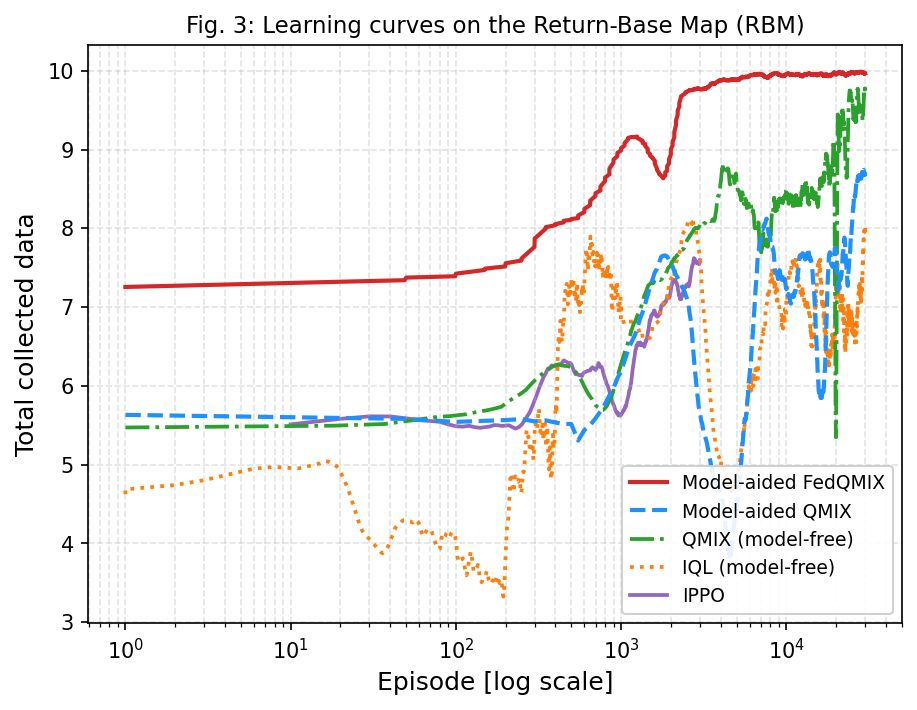
\includegraphics[width=0.88\linewidth]{RBM.jpeg}
  \caption{Learning curves on the \emph{Return--Base Map} (RBM). Several methods reach near-ceiling localisation performance under the training setup, but FedQMIX remains among the strongest and most stable performers across seeds.}
  \label{fig:rbm_learning_curve}
\end{figure}

\begin{figure}[H]
  \centering
  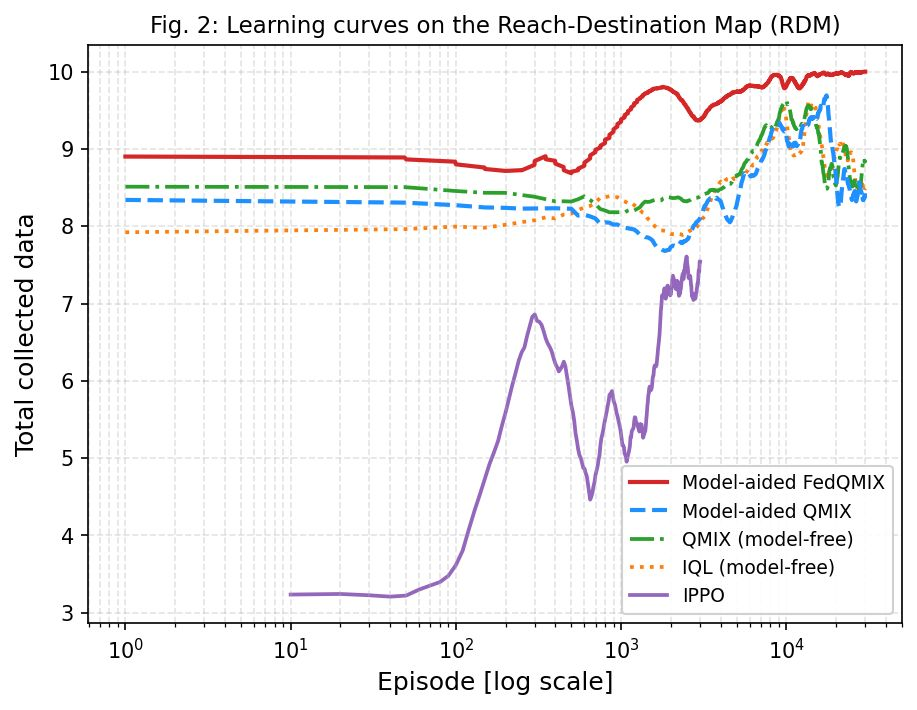
\includegraphics[width=0.88\linewidth]{RDM.jpeg}
  \caption{Learning curves on the \emph{Reach--Destination Map} (RDM; $1000{\times}1200$~m urban grid). Curves show the mean number of distinct victims localised as a function of training progress. FedQMIX converges rapidly to near-ceiling performance and remains the most stable method across seeds in the more demanding long-horizon scenario.}
  \label{fig:rdm_learning_curve}
\end{figure}


\begin{table}[H]
\centering
\caption{RBM evaluation scores.}
\label{tab:evaluation_scores}
\scriptsize
\begin{tabularx}{\textwidth}{@{}lCCCCC@{}}
\toprule
\textbf{Method-Seed} & \textbf{Eval-5} & \textbf{Eval-4} & \textbf{Eval-3} & \textbf{Eval-2} & \textbf{Eval-1} \\
\midrule
IPPO-s1 & \textbf{9.4} & \textbf{9.2} & \textbf{9.6} & \textbf{8.2} & \textbf{9.6} \\
IPPO-s2 & 8.4 & 8.8 & 7.6 & 7.6 & 8.4 \\
IPPO-s3 & 5.4 & 6.0 & 5.8 & 6.8 & 6.2 \\
IPPO-s4 & 6.6 & 7.0 & 7.0 & 7.0 & 6.8 \\
IPPO-s5 & 7.8 & 8.0 & 8.0 & 7.4 & 8.2 \\
\midrule
IQL-s1 & 6.4 & 6.8 & 7.4 & 7.4 & 7.6 \\
IQL-s2 & \textbf{8.8} & 8.4 & 8.7 & 8.2 & 8.5 \\
IQL-s3 & \textbf{8.8} & 8.8 & 8.7 & 8.7 & 8.1 \\
IQL-s4 & 8.6 & \textbf{9.1} & \textbf{9.0} & \textbf{8.9} & \textbf{9.2} \\
IQL-s5 & \textbf{8.8} & 7.8 & 7.3 & 7.4 & 7.3 \\
\midrule
QMIX-s1 & \textbf{10.0} & \textbf{10.0} & \textbf{10.0} & 9.8 & \textbf{10.0} \\
QMIX-s2 & \textbf{10.0} & 9.8 & \textbf{10.0} & 9.8 & 9.6 \\
QMIX-s3 & 9.8 & \textbf{10.0} & \textbf{10.0} & \textbf{10.0} & \textbf{10.0} \\
QMIX-s4 & \textbf{10.0} & 9.6 & 9.8 & 9.6 & 9.8 \\
QMIX-s5 & 9.4 & \textbf{10.0} & 9.6 & 9.6 & \textbf{10.0} \\
\midrule
FED-s1 & 9.8 & \textbf{10.0} & \textbf{10.0} & 9.8 & \textbf{10.0} \\
FED-s2 & \textbf{10.0} & \textbf{10.0} & 9.8 & 9.8 & \textbf{10.0} \\
FED-s3 & \textbf{10.0} & \textbf{10.0} & \textbf{10.0} & \textbf{10.0} & \textbf{10.0} \\
FED-s4 & \textbf{10.0} & \textbf{10.0} & \textbf{10.0} & \textbf{10.0} & \textbf{10.0} \\
FED-s5 & 9.8 & \textbf{10.0} & \textbf{10.0} & \textbf{10.0} & \textbf{10.0} \\
\midrule
MOD-s1 & 9.0 & \textbf{9.0} & 8.2 & \textbf{9.4} & 8.8 \\
MOD-s2 & 9.0 & 8.8 & \textbf{9.0} & 9.0 & \textbf{9.0} \\
MOD-s3 & 8.0 & 8.0 & 8.0 & 8.0 & 8.0 \\
MOD-s4 & \textbf{9.2} & \textbf{9.0} & \textbf{9.0} & 9.0 & \textbf{9.0} \\
MOD-s5 & 8.0 & 8.4 & 8.0 & 8.2 & \textbf{9.0} \\
\bottomrule
\end{tabularx}
\end{table}

\begin{table}[H]
\centering
\caption{RDM evaluation scores.}
\label{tab:rdm-evals}
\scriptsize
\begin{tabularx}{\textwidth}{@{}lCCCCC@{}}
\toprule
\textbf{Method-Seed} & \textbf{Eval-5} & \textbf{Eval-4} & \textbf{Eval-3} & \textbf{Eval-2} & \textbf{Eval-1} \\
\midrule
IPPO-s1 & 8.2 & 9.2 & 9.4 & 8.6 & 8.0 \\
IPPO-s2 & 5.0 & 5.0 & 5.0 & 5.0 & 5.0 \\
IPPO-s3 & 7.2 & 7.0 & 7.0 & 7.2 & 7.4 \\
IPPO-s4 & \textbf{10.0} & \textbf{9.8} & \textbf{9.6} & \textbf{9.8} & \textbf{9.6} \\
IPPO-s5 & 7.4 & 7.4 & 7.8 & 8.0 & 6.4 \\
\midrule
IQL-s1 & 7.0 & 7.0 & 8.4 & 7.2 & 6.8 \\
IQL-s2 & 7.0 & 7.2 & 7.0 & 7.2 & 7.4 \\
IQL-s3 & \textbf{9.8} & 9.6 & 9.2 & \textbf{10.0} & \textbf{9.6} \\
IQL-s4 & 9.4 & 8.6 & 8.6 & 7.8 & \textbf{9.6} \\
IQL-s5 & \textbf{9.8} & \textbf{9.8} & \textbf{9.8} & 9.6 & \textbf{9.6} \\
\midrule
QMIX-s1 & \textbf{9.9} & \textbf{10.0} & \textbf{10.0} & \textbf{10.0} & \textbf{10.0} \\
QMIX-s2 & 8.2 & 8.3 & 8.2 & 8.2 & 8.1 \\
QMIX-s3 & 8.1 & 7.2 & 7.7 & 8.2 & 8.0 \\
QMIX-s4 & 8.2 & 8.4 & 8.3 & 8.4 & 8.1 \\
QMIX-s5 & \textbf{9.9} & 9.8 & 9.6 & 9.9 & 9.8 \\
\midrule
FED-s1 & 9.9 & \textbf{10.0} & \textbf{10.0} & \textbf{10.0} & \textbf{10.0} \\
FED-s2 & \textbf{10.0} & \textbf{10.0} & \textbf{10.0} & \textbf{10.0} & \textbf{10.0} \\
FED-s3 & \textbf{10.0} & \textbf{10.0} & \textbf{10.0} & \textbf{10.0} & \textbf{10.0} \\
FED-s4 & \textbf{10.0} & \textbf{10.0} & \textbf{10.0} & \textbf{10.0} & \textbf{10.0} \\
FED-s5 & \textbf{10.0} & \textbf{10.0} & \textbf{10.0} & \textbf{10.0} & \textbf{10.0} \\
\midrule
MOD-s1 & 7.0 & 9.4 & 7.0 & 7.0 & 9.3 \\
MOD-s2 & \textbf{9.4} & \textbf{10.0} & \textbf{9.8} & \textbf{9.4} & 9.7 \\
MOD-s3 & 8.8 & 8.8 & 8.6 & 7.4 & 9.1 \\
MOD-s4 & 8.0 & 8.3 & 8.0 & 8.0 & 8.8 \\
MOD-s5 & 9.1 & 9.4 & 8.8 & 8.8 & \textbf{9.9} \\
\bottomrule
\end{tabularx}
\end{table}

\paragraph{Statistical protocol.}
To reduce the effect of stochastic beacon emissions and seed-level variability,
all main comparisons are reported across five independent seeds per method and map.
For summary comparisons we report mean and standard deviation across seeds.
Using the common seed set across methods, we further report paired one-sided
Wilcoxon signed-rank tests against FedQMIX and Cliff's $\delta$ effect sizes at the
final evaluation checkpoint. Given the modest sample size, these statistics should
be interpreted together with effect sizes and ceiling effects, but they provide
substantially stronger evidence than the earlier three-seed configuration.

\paragraph{Baseline choice and interpretation.}
Our baseline set covers both standard model-free MARL methods and more structured
alternatives. Independent Q-Learning (IQL) represents independent value-based agents
with decentralised training, while QMIX provides a strong centralised-training,
decentralised-execution value-factorisation baseline. IPPO supplies a policy-gradient
actor--critic comparator. Model-Aided QMIX (MOD) uses the same surrogate channel and
PSO-based localisation module as FedQMIX but removes federation, isolating the value
of parameter sharing from the value of model guidance. Finally, the deterministic
coverage heuristic represents a classical SAR-style sweep baseline that prioritises
eventual area coverage rather than adaptive information gathering.


\paragraph{RBM performance.}
Table~\ref{tab:evaluation_scores} reports the number of distinct victims localised on
the $600{\times}800$\,m RBM. In this compact map, several methods approach the
10-victim ceiling under the reward and training setup. The strongest two
methods are \textsc{FED} and \textsc{QMIX}, both of which repeatedly achieve
near-ceiling or ceiling-level scores across the final checkpoints. In particular,
FedQMIX remains highly consistent across all five seeds, with final scores of
9.8--10.0, while QMIX also performs strongly but exhibits slightly broader variation
across seeds and checkpoints. MOD remains competitive but below the top two methods,
whereas IQL and IPPO improve substantially relative to the earlier version yet still
show greater variability and lower average performance. Overall, RBM behaves as a
comparatively easier, partially saturated regime in which several methods can attain
high final localisation, but FedQMIX remains among the strongest and most stable.


\paragraph{RDM performance.}
Table~\ref{tab:rdm-evals} summarises the $1000{\times}1200$\,m RDM results. In
contrast to RBM, RDM remains more discriminative and therefore provides the clearest
comparison between methods. FedQMIX is the strongest and most stable method across the
entire table: four seeds achieve perfect final scores of 10.0 and the fifth reaches
9.9, with all seeds remaining at or extremely near the ceiling across the last five
evaluation checkpoints. QMIX contains both very strong and substantially weaker seeds,
indicating higher sensitivity to training variation. IQL and MOD remain competitive in
their best cases but do not match the consistency of FedQMIX across seeds. IPPO
exhibits the largest cross-seed variability, with one near-ceiling seed and several
substantially weaker runs. Thus, RDM provides the strongest evidence that federated
parameter sharing and model-aided guidance improve both final localisation performance
and cross-seed robustness in the more demanding long-horizon setting.


\paragraph{Final performance summary.}
Table~\ref{tab:final_summary} summarises the final evaluation performance at
\texttt{Eval-5} across five seeds. FedQMIX achieves the highest mean score on both
maps and also exhibits the lowest cross-seed variance, especially on RDM, where it
reaches near-perfect and highly stable localisation. On RBM, both FED and QMIX operate
close to the 10-victim ceiling, indicating partial saturation of the easier scenario.
On the more discriminative RDM map, however, FedQMIX retains a clear advantage in both
average performance and robustness.


\begin{table}[H]
\centering
\caption{Final evaluation summary across five seeds (Eval-5). Values are reported as mean $\pm$ standard deviation of distinct victims localised.}
\label{tab:final_summary}
\begin{tabularx}{\textwidth}{@{}lCC@{}}
\toprule
\textbf{Method} & \textbf{RBM Eval-5} & \textbf{RDM Eval-5} \\
\midrule
IPPO & $7.52 \pm 1.56$ & $7.56 \pm 1.81$ \\
IQL  & $8.28 \pm 1.05$ & $8.60 \pm 1.47$ \\
QMIX & $9.84 \pm 0.26$ & $8.86 \pm 0.95$ \\
FED  & $\mathbf{9.92 \pm 0.11}$ & $\mathbf{9.98 \pm 0.04}$ \\
MOD  & $8.64 \pm 0.59$ & $8.46 \pm 0.97$ \\
\bottomrule
\end{tabularx}
\end{table}



\paragraph{Statistical comparison against FedQMIX.}
Table~\ref{tab:stat_comparison} confirms that FedQMIX achieves the strongest overall
final performance across both maps. On RBM, the difference between FED and QMIX is
small, which is consistent with the ceiling effect observed in the easier return-to-base
scenario; accordingly, Cliff's $\delta$ is close to zero and the paired Wilcoxon test
does not indicate a clear separation. In contrast, FED shows large or maximal effect
sizes against IPPO, IQL, and MOD on RBM. On RDM, where the task is more discriminative,
FED maintains both the highest mean performance and markedly stronger effect sizes than
all baselines, with especially clear separation from IQL and MOD. These results support
the interpretation that the main empirical advantage of FedQMIX lies not only in high
final localisation performance, but also in stronger robustness across seeds, especially
in the more demanding long-horizon scenario.


\begin{table}[H]
\centering
\caption{Statistical comparison against FedQMIX at the final evaluation checkpoint (Eval-5). Values are reported as mean $\pm$ standard deviation of distinct victims localised across five seeds. Cliff's $\delta$ is computed relative to FED, with positive values favouring FED. The reported $p$-values are from paired one-sided Wilcoxon signed-rank tests using the common seed set across methods.}
\label{tab:stat_comparison}
\scriptsize
\setlength{\tabcolsep}{4pt}
\begin{tabularx}{\textwidth}{@{}lCCCCC@{}}
\toprule
\textbf{Method} & \textbf{RBM mean $\pm$ std} & \textbf{RDM mean $\pm$ std} & \textbf{RBM $\delta$} & \textbf{RDM $\delta$} & \textbf{$p$-value (RBM / RDM)} \\
\midrule
IPPO & $7.52 \pm 1.56$ & $7.56 \pm 1.81$ & $1.00$ & $0.76$ & $0.0313$ / $0.0625$ \\
IQL  & $8.28 \pm 1.05$ & $8.60 \pm 1.47$ & $1.00$ & $1.00$ & $0.0313$ / $0.0313$ \\
QMIX & $9.84 \pm 0.26$ & $8.86 \pm 0.95$ & $0.08$ & $0.92$ & $0.3750$ / $0.0625$ \\
MOD  & $8.64 \pm 0.59$ & $8.46 \pm 0.97$ & $1.00$ & $1.00$ & $0.0313$ / $0.0313$ \\
FED  & $\mathbf{9.92 \pm 0.11}$ & $\mathbf{9.98 \pm 0.04}$ & -- & -- & -- \\
\bottomrule
\end{tabularx}
\end{table}

\paragraph{Overall comparison.}
Taken together, Tables~\ref{tab:evaluation_scores} and~\ref{tab:rdm-evals}
show that the FedQMIX pipeline is the strongest and most stable overall
performer across the two operational regimes. On RBM, several methods reach the
ceiling region, making the scenario partly saturated; on RDM, however, the advantage
of FedQMIX becomes much clearer in both mean performance and consistency. This pattern
supports the interpretation that federation and model guidance are especially valuable
when the search problem is longer-horizon, less forgiving, and more sensitive to early
coordination errors.

\noindent\textbf{Learning-curve analysis.}
Figures~\ref{fig:rbm_learning_curve} and~\ref{fig:rdm_learning_curve} complement the
final checkpoint tables by showing the full learning dynamics. On RBM, the
reward and training setup allow several methods to approach ceiling performance, so the
main distinction is not whether high performance is reached, but how smoothly and how
consistently it is maintained across seeds. FedQMIX reaches the high-performance region
rapidly and remains stable thereafter. On RDM, the curves are more clearly separated:
FedQMIX rises quickly and stays near the 10-victim ceiling across seeds, whereas the
competing baselines show either slower improvement, larger fluctuations, or stronger
seed dependence. Thus, the learning curves reinforce the same qualitative conclusion as
the final tables: the FedQMIX framework provides the strongest balance of
sample efficiency, final performance, and robustness, especially in the harder RDM
scenario.



\begin{figure}[!t]
  \centering
  \includegraphics[width=.55\linewidth]{legend_box_3x3.png}\par\vspace{6pt}
  \begin{subfigure}[t]{.47\linewidth}
      \centering
      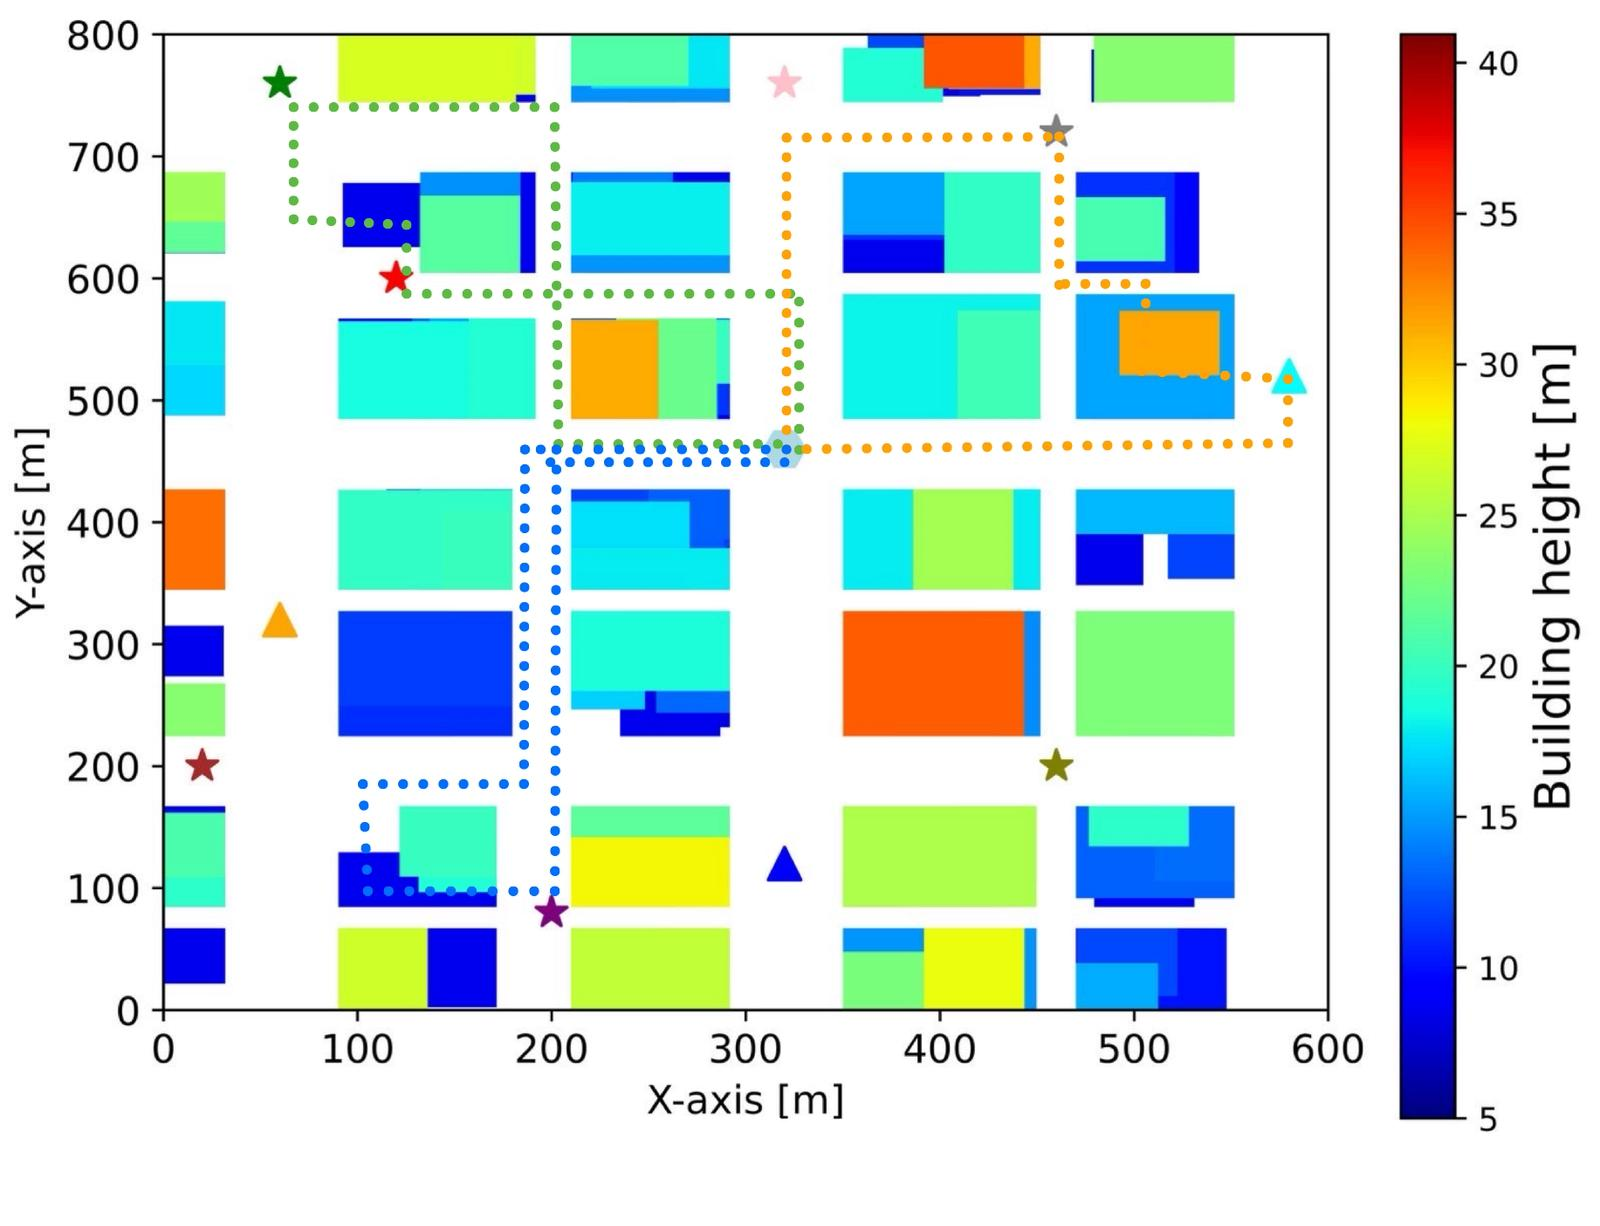
\includegraphics[width=\linewidth]{RBM_map.jpeg}
      \caption{Return-Base Map (RBM)}\label{fig:rbm_panel}
  \end{subfigure}\hfill
  \begin{subfigure}[t]{.47\linewidth}
      \centering
      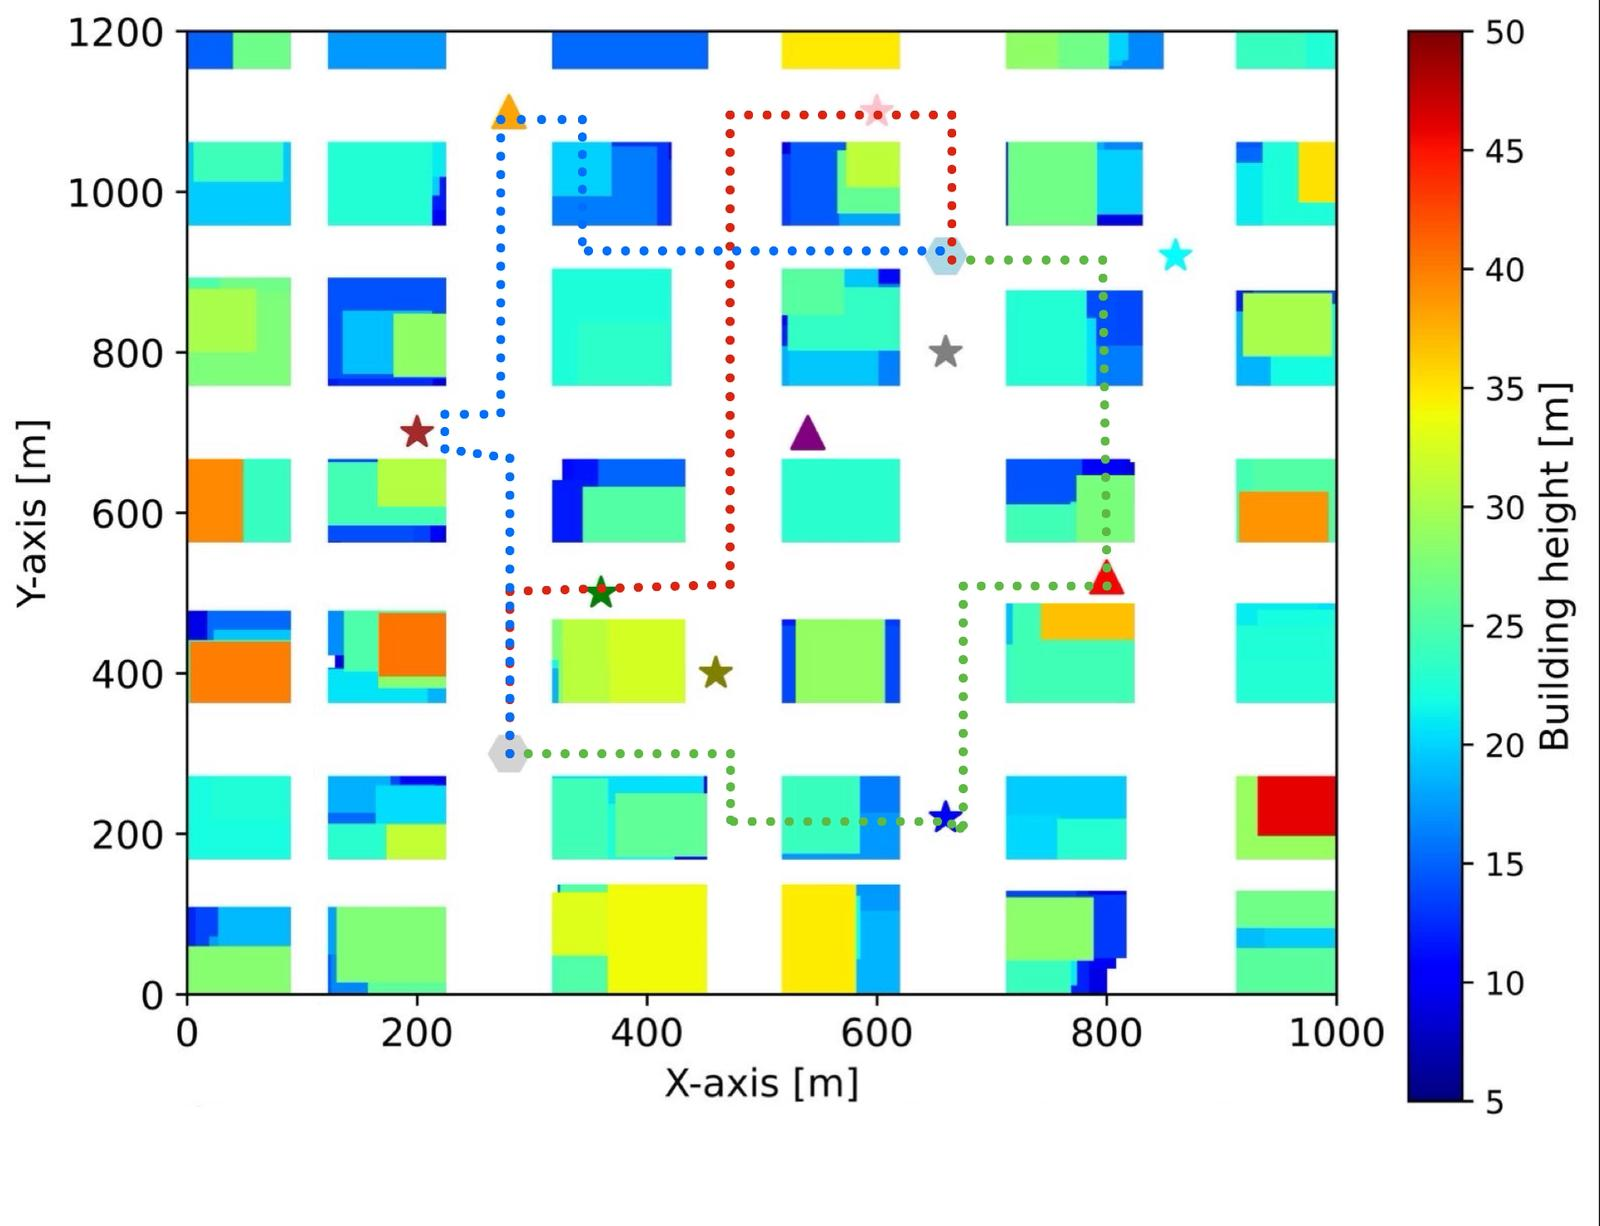
\includegraphics[width=\linewidth]{RDM_map.jpeg}
      \caption{Reach-Destination Map (RDM)}\label{fig:rdm_panel}
  \end{subfigure}
  \caption{Illustration of the two simulated post-disaster urban environments:
(a) RBM ($600{\times}800$ m) and
(b) RDM ($1000{\times}1200$ m).
The coloured background shows the building/rubble height map $H(x,y)$.
Stars mark victim devices, triangles denote anchor beacons, shaded rectangles indicate UAV
start and terminal zones, and dotted lines show example UAV trajectories.
For visual clarity, only three UAV trajectories are shown, although all experiments use $I=4$ UAVs.}
  \label{fig:paths_two_maps}
\end{figure}

\paragraph{Ablation on surrogate channel and federation.}
To isolate the contributions of the radio-channel surrogate and federated parameter
sharing, we also consider a $2\times2$ ablation over FedQMIX variants with federation
on/off and surrogate channel on/off. Table~\ref{tab:ablation} reports the corresponding
diagnostic results. When the surrogate is disabled, federation improves victim
localisation on both maps, supporting the claim that cross-client parameter sharing is
a major contributor to stability and final performance. When the surrogate is enabled,
final localisation counts are lower overall, which should not be interpreted as evidence
against the surrogate; rather, it reflects the fact that the learned LoS/NLoS model
introduces a more realistic and therefore harder optimisation environment. We therefore
interpret the surrogate primarily as a realism and transfer mechanism, whose main value
lies in reducing optimism bias and producing more physically grounded learning dynamics,
rather than simply maximising scores under idealised signal assumptions.

\begin{table}[htbp]
\centering
\caption{Ablation on surrogate channel and federation for FedQMIX.
Entries report mean $\pm$ standard deviation of distinct victims localised
over three seeds after 1000 training episodes per configuration.}
\label{tab:ablation}
\begin{tabular*}{\linewidth}{@{\extracolsep{\fill}} lccc}
\toprule
\textbf{Map} & \textbf{Federation} & \textbf{Surrogate} & \textbf{Victims localised} \\
\midrule
\multirow{4}{*}{RBM}
  & off & off & $7.31 \pm 1.04$ \\
  & off & on  & $6.07 \pm 2.49$ \\
  & on  & off & $\mathbf{9.25} \pm 0.70$ \\
  & on  & on  & $6.28 \pm 2.99$ \\
\midrule
\multirow{4}{*}{RDM}
  & off & off & $9.05 \pm 0.66$ \\
  & off & on  & $8.20 \pm 0.72$ \\
  & on  & off & $\mathbf{9.60} \pm 0.53$ \\
  & on  & on  & $8.17 \pm 0.84$ \\
\bottomrule
\end{tabular*}
\end{table}

\paragraph{Coverage heuristic baseline.}
We also evaluated a deterministic coverage (“lawnmower”) heuristic under the same
episode settings as the main experiments. In each episode, victim devices were
randomly deactivated according to a Bernoulli on/off model ($p_{\text{on}}=0.8$), and
the heuristic executed a precomputed sweep without learning. To avoid
pseudo-replication across 200 episodes per seed, we first computed per-seed summaries
(episode-level means and medians for first-detection metrics) and then reported the
mean $\pm$ standard deviation across seeds.

Table~\ref{tab:coverage_heuristic_summary} shows that the coverage heuristic achieves
near-complete coverage on both maps (mean completion $\approx 0.98$ for RBM and $1.00$
for RDM), with an average of $\sim 7.84$ victims detected per episode in RBM and
$\sim 7.98$ in RDM. The first detection occurs earlier on RBM (FirstT mean
$\approx 3.68$ steps) than on RDM (FirstT mean $\approx 9.13$ steps), consistent with
the larger and more diffuse RDM layout. Energy usage is also higher in RDM
($\sim 211.63$) than RBM ($\sim 143.42$). Median energy-to-first-detection
(FirstE med) is $12.00$ in RBM and $24.00$ in RDM, aligning with the corresponding
first-detection medians and the environment energy accounting.

\begin{table}[htbp]
\centering
\caption{Coverage heuristic baseline results. Seed-level summaries (5 RBM + 5 RDM) and final aggregation (mean $\pm$ standard deviation across seeds).}
\label{tab:coverage_heuristic_summary}

\scriptsize
\setlength{\tabcolsep}{2.5pt}
\renewcommand{\arraystretch}{1.05}

\subcaption*{Seed-level summary (5 RBM + 5 RDM)}
\begin{tabular*}{\linewidth}{@{\extracolsep{\fill}} l rr rr r r r}
\toprule
\multirow{2}{*}{Map/Seed} &
  \multicolumn{2}{c}{Vict.} &
  \multicolumn{2}{c}{FirstT} &
  \multirow{2}{*}{FirstE med} &
  \multirow{2}{*}{Energy mean} &
  \multirow{2}{*}{Compl.\ mean} \\
\cmidrule(lr){2-3}\cmidrule(lr){4-5}
 & mean & std & med & mean & & & \\
\midrule
RBM1 & 7.68 & 1.37 & 4.00 & 3.75 & 12.00 & 142.28 & 0.98 \\
RBM2 & 7.91 & 1.26 & 4.00 & 3.73 & 12.00 & 141.81 & 0.99 \\
RBM3 & 7.91 & 1.25 & 4.00 & 3.65 & 12.00 & 143.72 & 0.98 \\
RBM4 & 7.83 & 1.15 & 4.00 & 3.61 & 12.00 & 143.49 & 0.98 \\
RBM5 & 7.82 & 1.28 & 4.00 & 3.72 & 12.00 & 141.47 & 0.98 \\
RDM1 & 7.84 & 1.40 & 8.00 & 9.20 & 24.00 & 211.10 & 1.00 \\
RDM2 & 8.03 & 1.28 & 8.00 & 8.66 & 24.00 & 210.74 & 1.00 \\
RDM3 & 8.05 & 1.25 & 8.00 & 9.53 & 24.00 & 211.88 & 1.00 \\
RDM4 & 7.97 & 1.19 & 8.00 & 9.48 & 24.00 & 211.98 & 1.00 \\
RDM5 & 7.96 & 1.30 & 8.00 & 8.70 & 24.00 & 211.08 & 1.00 \\
\bottomrule
\end{tabular*}

\vspace{0.6em}

\subcaption*{Final (mean across seeds $\pm$ std across seeds)}
\begin{tabular*}{\linewidth}{@{\extracolsep{\fill}} l rr rr r r r r}
\toprule
\multirow{2}{*}{Map} &
  \multicolumn{2}{c}{Vict.} &
  \multicolumn{2}{c}{FirstT} &
  \multirow{2}{*}{FirstT med} &
  \multirow{2}{*}{FirstE med} &
  \multirow{2}{*}{Energy mean} &
  \multirow{2}{*}{Compl.\ mean} \\
\cmidrule(lr){2-3}\cmidrule(lr){4-5}
 & mean & std & mean & std & & & & \\
\midrule
RBM & 7.84 & 0.10 & 3.68 & 0.05 & 4.00 & 12.00 & 143.42 & 0.98 \\
RDM & 7.98 & 0.08 & 9.13 & 0.29 & 8.00 & 24.00 & 211.63 & 1.00 \\
\bottomrule
\end{tabular*}
\end{table}

\paragraph{Sensitivity to $p_{\mathrm{on}}$, $\mathrm{SNR}_{\mathrm{thr}}$, and safety radius.}
Table~\ref{tab:sensitivity} reports a small sensitivity sweep around the nominal
Model-Aided FedQMIX configuration. On the compact RBM map, the method localises
approximately 3.7--4.3 victims across all settings; the main effect is a modest
improvement when the BLE duty cycle is reduced from $p_{\mathrm{on}}=0.8$ to
$p_{\mathrm{on}}=0.6$ (4.33 vs.\ 3.67 victims), accompanied by a reduction in energy
per victim from $\approx 147$ to $\approx 125$ units. Changing the SNR threshold by
5\,dB (from $0$ to $-5$\,dB) and doubling the safety radius (from $R=3$ to $R=6$
cells) has negligible impact on final performance in this smaller scene.
On the larger RDM map, the policy operates close to the 10-victim upper bound for all
tested settings (9.0--10.0 victims), and energy per victim varies only mildly
(72--80 units). The best RDM configuration is obtained for the stricter spatial
separation $R=6$, where FedQMIX still recovers all victims. Overall, within the
practically relevant range explored here, FedQMIX appears robust: moderate changes in
intermittency, channel quality, and safety radius do not qualitatively alter
localisation performance or energy efficiency. Because full multi-seed sensitivity
experiments are computationally expensive, the sensitivity analysis should be read as
qualitative rather than as formal statistical evidence.

\begin{table}[t]
\centering
\caption{Sensitivity of Model-Aided FedQMIX to BLE duty cycle, SNR threshold,
and safety radius. Each row corresponds to one configuration evaluated
with a single seed. Metrics report mean victims localised and mean energy
per victim over evaluation episodes.}
\label{tab:sensitivity}
\begin{tabular*}{\linewidth}{@{\extracolsep{\fill}} l c c c c c c}
\toprule
\textbf{Map} & \textbf{BLE duty cycle} & \textbf{SNR thr. [dB]} & \textbf{$R$ [cells]} &
\textbf{Seeds} & \textbf{Mean victims} & \textbf{Energy} \\
\midrule
RBM & 0.60 & 0  & 3 & 1 & 4.33 & 124.62 \\
RBM & 0.80 & -5 & 3 & 1 & 3.67 & 147.27 \\
RBM & 0.80 & 0  & 3 & 1 & 3.67 & 147.27 \\
RBM & 0.80 & 0  & 6 & 1 & 3.67 & 147.27 \\
\midrule
RDM & 0.60 & 0  & 3 & 1 & 9.33 & 77.14 \\
RDM & 0.80 & -5 & 3 & 1 & 9.00 & 80.00 \\
RDM & 0.80 & 0  & 3 & 1 & 9.67 & 74.48 \\
RDM & 0.80 & 0  & 6 & 1 & 10.00 & 72.00 \\
\bottomrule
\end{tabular*}
\end{table}

%======================================================================%
\subsection{Deployment-Oriented Federated Coordination Considerations}
\label{sec:deployment}
%======================================================================%

Although the federated learning primitive in our pipeline uses standard FedAvg
(Eqs.~\eqref{eq:fedavg} and \eqref{eq:fedavg2}), its operational viability in
post-disaster SAR depends on two practical questions: \emph{(i)} whether parameter
exchange fits within bandwidth-limited and intermittent air-to-air links, and
\emph{(ii)} whether the privacy boundary is acceptable when multiple agencies
collaborate.

\paragraph{Communication payload and link feasibility.}
Let $d_\theta$ denote the number of trainable parameters exchanged per FedAvg round
(QMIX agents and mixing network). With 32-bit floats, each client transmits
$S_{\text{up}} = 4d_\theta$ bytes uplink and receives $S_{\text{down}} = 4d_\theta$
bytes downlink. In our implementation, $d_\theta \approx 1.2\times 10^5$, giving
$S_{\text{up}} \approx S_{\text{down}} \approx 0.46$\,MB per round. Given the
aggregation period $N_{\text{freq}}=50$ episodes between rounds, the average link
utilisation remains modest: under a 200\,kbps air-to-air link, the end-to-end
parameter exchange corresponds to under $\sim 3\%$ of link capacity. This indicates
that standard FedAvg can be feasible even when SAR communications are degraded, as
long as aggregation is not triggered too frequently. Additional compression
(e.g., 16-bit quantisation) can further halve this payload without changing the
training logic.

\paragraph{Privacy boundary and threat model.}
The pipeline is designed to keep raw operational traces on-board each UAV. In
particular, the following sensitive data remain local: flight trajectories, per-step
RSSI logs, per-victim contact histories, and local replay buffers. Only model
parameters are exchanged. This reduces the risk of exposing victim-related signal
traces or operational flight paths that could be sensitive under multi-agency or
multi-jurisdictional SAR deployments. We emphasise that federated learning does not
guarantee absolute privacy, but it substantially narrows the shared information
surface compared with centralised logging.

\paragraph{Guidelines for intermittent connectivity.}
Real SAR links can be intermittent due to obstruction, congestion, or energy-saving
radio duty cycling. The federated loop can be made robust without changing its core
logic by:
\emph{(i)} caching local updates on-board and uploading them when connectivity is
restored (delayed aggregation),
\emph{(ii)} allowing partial client participation, where the aggregator averages only
the available subset of clients in a given round, and
\emph{(iii)} falling back to locally trained policies when the aggregator is
temporarily unreachable. These protocol considerations are critical for translating
simulation-heavy FRL pipelines into field deployments where strict, continuous
connectivity cannot be assumed.


%\FloatBarrier





\section{Conclusion and Limitations}
\label{sec13}

This study examined whether a \emph{model-aided, federated multi-agent RL}
pipeline can provide a practically meaningful basis for post-disaster UAV victim
localisation under partial observability, communication constraints, and safety
requirements. The proposed framework combines a lightweight LoS/NLoS channel
surrogate, PSO-based victim position estimation, a SAR-aligned shaped reward,
a leakage-free global training state based on estimated victim locations, and a
federated QMIX backbone that exchanges parameters rather than raw operational data.

Across two post-earthquake urban maps representing distinct operational regimes,
the proposed FedQMIX framework emerged as the strongest and most stable overall
performer. On the compact RBM scenario, several methods approached the
10-victim ceiling under the shaped reward design, indicating that this map is
partially saturated and therefore less discriminative among top-performing
methods. Even in this setting, however, FedQMIX remained among the strongest and
most consistent methods across seeds. On the larger and more demanding RDM
scenario, the advantage of FedQMIX became substantially clearer: it achieved
near-perfect final localisation performance with the lowest cross-seed variance,
outperforming IQL, IPPO, and the non-federated model-aided baseline, while also
showing stronger stability than model-free QMIX. Taken together, these results
suggest that the main empirical strength of the proposed framework lies not only
in strong final victim-localisation performance, but also in robustness under
more difficult long-horizon coordination conditions.

Beyond final scores, the study contributes at the system-design level.
The SAR-aligned shaped reward reduces the mismatch between the training objective
and the mission-level evaluation criterion, the leakage-free state design removes
privileged ground-truth victim coordinates from centralised training, and the
deployment-oriented federated analysis clarifies the practical feasibility of
parameter sharing under bandwidth and privacy constraints. The communication
payload remains modest, the privacy boundary is substantially narrower than under
centralised logging, and delayed aggregation or partial participation can be
handled naturally within the deployment protocol. In this sense, the contribution
is not a novel aggregation rule in the strict algorithmic sense, but a more
deployment-conscious formulation of federated multi-agent coordination for SAR.

\paragraph{Scenario-dependent applicability.}
The two evaluation scenes correspond to different operational regimes, and the
benefits of the proposed framework manifest differently in each. In the compact,
dense \emph{Return--Base Map} (RBM), the UAV fleet starts and finishes near the
same base, so the main challenge is to rapidly cover the local area while
retaining enough energy to return safely. In this regime, the training setup
enables several methods to perform well, and the principal distinction is
therefore one of stability and smoothness rather than raw asymptotic score.
In contrast, the \emph{Reach--Destination Map} (RDM) behaves like a longer
corridor under tighter energy constraints, where early miscoordination is much
more costly. In this setting, the combination of federated parameter sharing and
model-aided guidance is most valuable: FedQMIX maintains near-ceiling
performance across all seeds, whereas competing methods exhibit either larger
variance, slower convergence, or both. Thus, RBM mainly highlights that the
framework remains competitive in an easier, partially saturated regime,
whereas RDM provides the clearest evidence of its robustness and practical value
in more demanding long-horizon scenarios.

\paragraph{Limitations and robustness.}
Several simplifying assumptions delimit the scope of the present study.
First, victims are assumed to be static and to emit BLE beacons with a fixed,
homogeneous probability; in reality, survivors may move, change device
orientation or power state, or be temporarily shielded by rescuers, vehicles, or
dynamic obstructions. Second, the BLE surrogate captures only a simplified
LoS/NLoS log-distance structure and does not explicitly model device-specific
hardware variability, antenna patterns, or extreme multipath outside the
training distribution. Third, the energy model abstracts propulsion, hovering,
and communication costs into discrete units and neglects effects such as wind,
payload differences, and battery ageing. Fourth, although the federated
framework is analysed from a deployment perspective, temporary communication
failures, delayed aggregation, and partial client participation are not yet
explicitly simulated in the main experiments. Fifth, the environments are
synthetic and stylised rather than field-calibrated rubble scenes, and the
surrogate is trained on simulated anchor measurements rather than mixed
simulated-and-measured traces.

The main experiments are reported across five independent seeds per method and
map, and the final-checkpoint analysis is supplemented with paired
nonparametric tests and Cliff's $\delta$ effect sizes. Even so, the sample size
remains modest, and the statistical results should be interpreted together with
ceiling effects, especially on RBM, where several methods approach saturation.
In addition, the ablation and sensitivity studies cover a narrower subset of
scenarios and hyperparameters than the main comparison, and should therefore be
interpreted more cautiously. Despite these limitations, the experiments show
qualitatively consistent trends across maps and seeds, supporting the robustness
of the main conclusions within the simulated regime considered here.

\paragraph{Physical validation perspective.}
Regarding the lack of physical real-world drone experiments, the present
study is intentionally positioned as a simulation-based methodological
and system-design study. Conducting a fully representative multi-UAV
post-disaster field experiment would require substantial logistical
preparation, dedicated test areas, safety permissions, multi-drone
coordination infrastructure, and controlled victim-beacon deployment,
which are beyond the scope of the current study. To mitigate this
limitation, we designed the simulation scenarios to reflect realistic
operational conditions, including obstruction-aware urban maps,
intermittent BLE beacon emissions, energy-constrained UAV motion,
TDMA-based communication constraints, and safety-feasible multi-UAV
coordination. The next stage of this research will therefore involve
controlled drone experiments in laboratory-scale or outdoor
rubble-inspired environments with BLE beacon targets, real onboard
communication constraints, and mission-level evaluation of victim
discovery time, localisation performance, and energy use. 

\paragraph{Path to deployment and ethics.}
Despite these limitations, the pipeline is designed to align with practical SAR
constraints. Federated training limits the amount of raw data---including
potentially sensitive RSSI traces, localisation histories, and flight
trajectories---that must leave each UAV, which is particularly important when
multiple agencies or jurisdictions collaborate. The safety layer enforces
altitude separation and return-to-base feasibility and can be extended to
include no-fly zones, human-specified corridors, or geofenced critical
infrastructure. A realistic deployment roadmap would first validate the
surrogate-learning and FedQMIX loop in a mock-city testbed, then in controlled
field exercises, before integrating it into incident-command workflows
alongside human operators and existing search procedures. Ethical deployment
also requires transparency about system limitations, conservative safety
margins, and explicit human oversight, especially when search priorities affect
the allocation of scarce rescue resources.

\paragraph{Federated-operation realism.}
Our simulations assume periodic parameter aggregation, but in practice SAR links
may be intermittent and the aggregator may be temporarily unreachable.
Importantly, this does not invalidate decentralised execution: each UAV can
continue to operate using its locally trained policy and upload cached updates
when connectivity returns. Partial participation and delayed aggregation should
therefore be viewed as natural operational modes of SAR deployment rather than
as algorithmic exceptions. Future work should explicitly simulate dropouts,
delayed rounds, and asynchronous aggregation so that the empirical analysis can
better reflect severe communication disruptions.

\paragraph{Future work.}
Several extensions follow directly from the above limitations. To relax the
static-victim assumption, future work should incorporate partially mobile
victims and more realistic device on/off patterns, and evaluate how FedQMIX
adapts when the target set evolves during the mission. To improve the radio
model, the LoS/NLoS surrogate should be calibrated on mixed
simulated-and-measured RSSI traces and extended to account for device
heterogeneity and body shadowing. On the dynamics side, the RL layer can be
coupled to richer propulsion and battery models, including wind fields, payload
effects, and explicit communication costs, and may benefit from risk-aware
objective functions that trade off localisation rate against safety or
communication uncertainty. From the federated-learning perspective, asynchronous
or event-triggered aggregation, robustness to partial participation, and
parameter compression deserve dedicated study. Finally, broader map families,
additional MARL and planning baselines, larger run ensembles, and ultimately a
multi-agency field exercise with real UAVs, BLE devices, and rubble testbeds
would help close the gap between simulation-heavy RL studies and operational SAR
systems.

%%%%%%%%%%%%%%%%%%%%%%%%%%%%%%%%%%%%%%%%%%
\vspace{6pt} 

%%%%%%%%%%%%%%%%%%%%%%%%%%%%%%%%%%%%%%%%%%
%% optional
%\supplementary{The following supporting information can be downloaded at:  \linksupplementary{s1}, Figure S1: title; Table S1: title; Video S1: title.}

% Only for journal Methods and Protocols:
% If you wish to submit a video article, please do so with any other supplementary material.
% \supplementary{The following supporting information can be downloaded at: \linksupplementary{s1}, Figure S1: title; Table S1: title; Video S1: title. A supporting video article is available at doi: link.}

% Only used for preprtints:
% \supplementary{The following supporting information can be downloaded at the website of this paper posted on \href{https://www.preprints.org/}{Preprints.org}.}

% Only for journal Hardware:
% If you wish to submit a video article, please do so with any other supplementary material.
% \supplementary{The following supporting information can be downloaded at: \linksupplementary{s1}, Figure S1: title; Table S1: title; Video S1: title.\vspace{6pt}\\
%\begin{tabularx}{\textwidth}{lll}
%\toprule
%\textbf{Name} & \textbf{Type} & \textbf{Description} \\
%\midrule
%S1 & Python script (.py) & Script of python source code used in XX \\
%S2 & Text (.txt) & Script of modelling code used to make Figure X \\
%S3 & Text (.txt) & Raw data from experiment X \\
%S4 & Video (.mp4) & Video demonstrating the hardware in use \\
%... & ... & ... \\
%\bottomrule
%\end{tabularx}
%}

%%%%%%%%%%%%%%%%%%%%%%%%%%%%%%%%%%%%%%%%%%
\authorcontributions{A. Guzey: conceptualization, methodology, formal analysis, writing original draft. M. A. Cifci: review, editing, and section-level refinement. A. Y. Erdogan: experimental execution and computational support.}

\funding{This research received no specific grant from any funding agency in the public, commercial, or not-for-profit sectors.}

\dataavailability{Simulation datasets (maps, RSSI traces, and replay buffers) are available from the corresponding author upon reasonable request. [Code availability:] Code is available from the corresponding author upon reasonable request. A public release is planned after publication.} 

%\durcstatement{Current research is limited to the [please insert a specific academic field, e.g., XXX], which is beneficial [share benefits and/or primary use] and does not pose a threat to public health or national security. Authors acknowledge the dual-use potential of the research involving xxx and confirm that all necessary precautions have been taken to prevent potential misuse. As an ethical responsibility, authors strictly adhere to relevant national and international laws about DURC. Authors advocate for responsible deployment, ethical considerations, regulatory compliance, and transparent reporting to mitigate misuse risks and foster beneficial outcomes.}

% Only for journal Nursing Reports
%\publicinvolvement{Please describe how the public (patients, consumers, carers) were involved in the research. Consider reporting against the GRIPP2 (Guidance for Reporting Involvement of Patients and the Public) checklist. If the public were not involved in any aspect of the research add: ``No public involvement in any aspect of this research''.}
%
%% Only for journal Nursing Reports
%\guidelinesstandards{Please add a statement indicating which reporting guideline was used when drafting the report. For example, ``This manuscript was drafted against the XXX (the full name of reporting guidelines and citation) for XXX (type of research) research''. A complete list of reporting guidelines can be accessed via the equator network: \url{https://www.equator-network.org/}.}
%
%% Only for journal Nursing Reports
%\useofartificialintelligence{Please describe in detail any and all uses of artificial intelligence (AI) or AI-assisted tools used in the preparation of the manuscript. This may include, but is not limited to, language translation, language editing and grammar, or generating text. Alternatively, please state that “AI or AI-assisted tools were not used in drafting any aspect of this manuscript”.}

%\acknowledgments{In this section you can acknowledge any support given which is not covered by the author contribution or funding sections. This may include administrative and technical support, or donations in kind (e.g., materials used for experiments). Where GenAI has been used for purposes such as generating text, data, or graphics, or for study design, data collection, analysis, or interpretation of data, please add “During the preparation of this manuscript/study, the author(s) used [tool name, version information] for the purposes of [description of use]. The authors have reviewed and edited the output and take full responsibility for the content of this publication.”}

\conflictsofinterest{The author declares no competing interests.} 

%%%%%%%%%%%%%%%%%%%%%%%%%%%%%%%%%%%%%%%%%%
%% Optional

%% Only for journal Encyclopedia
%\entrylink{The Link to this entry published on the encyclopedia platform.}
%
%\abbreviations{Abbreviations}{
%The following abbreviations are used in this manuscript:
%\\
%
%\noindent 
%\begin{tabular}{@{}ll}
%MDPI & Multidisciplinary Digital Publishing Institute\\
%DOAJ & Directory of open access journals\\
%TLA & Three letter acronym\\
%LD & Linear dichroism
%\end{tabular}
%}

%%%%%%%%%%%%%%%%%%%%%%%%%%%%%%%%%%%%%%%%%%
%% Optional
\appendixtitles{yes} % Leave argument "no" if all appendix headings stay EMPTY (then no dot is printed after "Appendix A"). If the appendix sections contain a heading then change the argument to "yes".
\appendixstart
\appendix

\section{Simulation Parameters}\label{app:params}

This appendix summarises the key simulation parameters used in the experiments.

\begin{table}[H]
\caption{Simulation parameters used throughout the study (nominal configuration, unless stated otherwise).}
\label{tab:sim-params}
\centering

\begin{adjustwidth}{-\extralength}{0cm}
\centering %% If there is a figure in wide page, please release command \centering, for Table, ``\textwidth" should be ``\fulllength"
\begin{tabularx}{\fulllength}{@{}lll@{}}
\toprule
\textbf{Parameter} & \textbf{Symbol / Value} & \textbf{Description} \\
\midrule
\multicolumn{3}{@{}l}{\textit{Environment / Map}} \\
\quad Horizontal size & RBM: $600\times800$\,m;\; RDM: $1000\times1200$\,m & Urban rubble bounds \\
\quad Vertical limit   & $Z_{\max}=30$\,m & Max debris/building height \\
\quad Grid resolution  & $\delta = 5$\,m & Cell size in $x$--$y$ plane \\
\quad Flyable region   & $\mathcal{F}$ & Voxels with $z>H(x,y)$ \\[4pt]

\multicolumn{3}{@{}l}{\textit{Devices / Channel}} \\
\quad Number of victim devices & $K=10$ & Trapped BLE devices (unknown) \\
\quad Nominal beacon duty       & $p_{\mathrm{on}}=0.8$ & Per-slot emission probability \\
\quad SNR threshold             & $\mathrm{SNR}_{\mathrm{thr}}=0$\,dB & Contact criterion (baseline) \\
\quad Tx/Noise powers           & $P,\;\sigma^{2}$ & Fixed within each experiment \\[4pt]

\multicolumn{3}{@{}l}{\textit{UAV Motion / Energy}} \\
\quad Number of UAVs   & $I=4$ & Fleet size \\
\quad Step length      & $c=5$\,m & Per-slot horizontal move \\
\quad Slot duration    & $\Delta t = 1$\,s & Time step \\
\quad Energy cost (hover/move) & $0.5/1.0$ (arb. units) & Used in~\eqref{eq:batt} \\
\quad Safety radius    & $R=3$ cells ($15$\,m) & Horizontal separation (baseline) \\[4pt]

\multicolumn{3}{@{}l}{\textit{Reward}} \\
\quad Communication reward & $r_t=\sum_{i,k} q_t^{i,k} C_t^{i,k}\Delta t$ & Eq.~\eqref{eq:reward} \\
\quad Shaped team reward & $\tilde r_t=\lambda_{\mathrm{thr}} r_t + \lambda_{\mathrm{new}}\Delta N_t^{\mathrm{new}}$ & Eq.~\eqref{eq:shaped_reward} \\[4pt]

\multicolumn{3}{@{}l}{\textit{Federated / Training}} \\
\quad Local sim.\ episodes    & $N=1000$ & Per deployment \\
\quad Fed.\ aggregation period & $N_{\text{freq}}=50$ & Episodes between FedAvg \\
\quad Target update period    & $N_{\text{target}}$ (hard) & As in Alg.~\ref{alg:FedQMIX} \\
\quad Max deployments         & $E_{\max}=30$ & Real-world rollouts \\
\quad Learning rate           & $5\times10^{-4}$ & Adam optimiser \\
\quad Batch size              & $B=32$ & Replay sampling \\
\quad Model size              & $d_\theta \approx 1.2\times10^{5}$ & QMIX parameters \\
\quad Payload / round         & $\approx 0.46$\,MB & $4d_\theta$ bytes at 32-bit \\
\bottomrule
\end{tabularx}
\end{adjustwidth}
\end{table}

%%%%%%%%%%%%%%%%%%%%%%%%%%%%%%%%%%%%%%%%%%
%\isPreprints{}{% This command is only used for ``preprints''.
\begin{adjustwidth}{-\extralength}{0cm}
%} % If the paper is ``preprints'', please uncomment this parenthesis.
%\printendnotes[custom] % Un-comment to print a list of endnotes

\reftitle{References}

% Please provide the correct journal abbreviation (e.g. according to the “List of Title Word Abbreviations” http://www.issn.org/services/online-services/access-to-the-ltwa/).
% Citations and References in Supplementary files are permitted provided that they also appear in the reference list here. 

%=====================================
% References, variant A: external bibliography
%=====================================
% \bibliography{your_external_BibTeX_file}
\bibliography{sn-bibliography}
%=====================================
% References, variant B: internal bibliography
%=====================================
%
%% ACS format
%\begin{thebibliography}{999}
%% Reference 1
%\bibitem{ref-journal}
%Author~1, T. The title of the cited article. {\em Journal Abbreviation} {\bf 2008}, {\em 10}, 142--149.
%% Reference 2
%\bibitem{ref-book1}
%Author~2, L. The title of the cited contribution. In {\em The Book Title}; Editor 1, F., Editor 2, A., Eds.; Publishing House: City, Country, 2007; pp. 32--58.
%% Reference 3
%\bibitem{ref-book2}
%Author 1, A.; Author 2, B. \textit{Book Title}, 3rd ed.; Publisher: Publisher Location, Country, 2008; pp. 154--196.
%% Reference 4
%\bibitem{ref-unpublish}
%Author 1, A.B.; Author 2, C. Title of Unpublished Work. \textit{Abbreviated Journal Name} year, \textit{phrase indicating stage of publication (submitted; accepted; in press)}.
%% Reference 5
%\bibitem{ref-url}
%Title of Site. Available online: URL (accessed on Day Month Year).
%% Reference 6
%\bibitem{ref-proceeding}
%Author 1, A.B.; Author 2, C.D.; Author 3, E.F. Title of presentation. In Proceedings of the Name of the Conference, Location of Conference, Country, Date of Conference (Day Month Year); Abstract Number (optional), Pagination (optional).
%% Reference 7
%\bibitem{ref-thesis}
%Author 1, A.B. Title of Thesis. Level of Thesis, Degree-Granting University, Location of University, Date of Completion.
%\end{thebibliography}

% If authors have biography, please use the format below
%\section*{Short Biography of Authors}
%\bio
%{\raisebox{-0.35cm}{\includegraphics[width=3.5cm,height=5.3cm,clip,keepaspectratio]{Definitions/author1.pdf}}}
%{\textbf{Firstname Lastname} Biography of first author}
%
%\bio
%{\raisebox{-0.35cm}{\includegraphics[width=3.5cm,height=5.3cm,clip,keepaspectratio]{Definitions/author2.jpg}}}
%{\textbf{Firstname Lastname} Biography of second author}

% For the MDPI journals use author-date citation, please follow the formatting guidelines on http://www.mdpi.com/authors/references
% To cite two works by the same author: \citeauthor{ref-journal-1a} (\citeyear{ref-journal-1a}, \citeyear{ref-journal-1b}). This produces: Whittaker (1967, 1975)
% To cite two works by the same author with specific pages: \citeauthor{ref-journal-3a} (\citeyear{ref-journal-3a}, p. 328; \citeyear{ref-journal-3b}, p.475). This produces: Wong (1999, p. 328; 2000, p. 475)

%%%%%%%%%%%%%%%%%%%%%%%%%%%%%%%%%%%%%%%%%%
%% for journal Sci
%\reviewreports{\\
%Reviewer 1 comments and authors’ response\\
%Reviewer 2 comments and authors’ response\\
%Reviewer 3 comments and authors’ response
%}
%%%%%%%%%%%%%%%%%%%%%%%%%%%%%%%%%%%%%%%%%%
\PublishersNote{}
%\isPreprints{}{% This command is only used for ``preprints''.
\end{adjustwidth}
%} % If the paper is ``preprints'', please uncomment this parenthesis.
\end{document}

